\documentclass[a4paper,12pt,abstracton,titlepage]{scrartcl}
\usepackage{scrpage2}
\usepackage[utf8]{inputenc}
\usepackage[T1]{fontenc}
\usepackage[top=2.5cm, bottom=2.5cm, left=2cm, right=2cm]{geometry}
\usepackage[affil-it]{authblk}
\usepackage{lipsum}
\usepackage{url}
\usepackage[hidelinks]{hyperref}
\usepackage{graphicx}
\usepackage[table,xcdraw]{xcolor}
\usepackage{longtable}
\usepackage{multicol}
\usepackage[toc,page]{appendix}

% header
\pagestyle{scrheadings}
\setheadsepline{0.2pt}
\clearscrheadings
\automark[section]{chapter}
\ihead{D.S.C. Schiavini and M. Baertsoen}
\ohead{Useful feedback in the Ampersand parser}
\cfoot{\pagemark}

% code listings
\usepackage{listings}
\usepackage{color}

\definecolor{mygreen}{rgb}{0,0.6,0}
\definecolor{mygray}{rgb}{0.5,0.5,0.5}
\definecolor{mymauve}{rgb}{0.58,0,0.82}
\lstset{%
    basicstyle=\small\ttfamily,
    breakatwhitespace=true,          % sets if automatic breaks should only happen at whitespace
    breaklines=true,                 % sets automatic line breaking
    commentstyle=\color{mygreen},    % comment style
    keepspaces=true,                 % keeps spaces in text, useful for keeping indentation of code (possibly needs columns=flexible)
    keywordstyle=\color{blue},       % keyword style
    numbersep=5pt,                   % how far the line-numbers are from the code
    numberstyle=\tiny\color{mygray}, % the style that is used for the line-numbers
    stepnumber=1,                    % the step between two line-numbers. If it's 1, each line will be numbered
    stringstyle=\color{mymauve},     % string literal style
}

\lstnewenvironment{haskell}{\lstset{language=Haskell,numbers=left, otherkeywords={}, deletekeywords={}}}{}
\lstnewenvironment{adl}{\lstset{language=Haskell,numbers=left, otherkeywords={INCLUDE,CONTEXT,ENDCONTEXT,EXTENDS,THEMES,META,PATTERN,ENDPATTERN,PROCESS,ENDPROCESS,INTERFACE,CLASS,FOR,BOX,ROWS,TABS,COLS,INITIAL,SQLPLUG,PHPPLUG,TYPE,POPULATION,CONTAINS,UNI,INJ,SUR,TOT,SYM,ASY,TRN,RFX,IRF,AUT,PROP,ALWAYS,RULE,MESSAGE,VIOLATION,SRC,TGT,TEST,RELATION,MEANING,CONCEPT,IDENT,VIEW,ENDVIEW,DEFAULT,TXT,PRIMHTML,TEMPLATE,KEY,IMPORT,SPEC,ISA,IS,I,V,CLASSIFY,PRAGMA,PURPOSE,IN,REF,ENGLISH,DUTCH,REST,HTML,LATEX,MARKDOWN,ONE,BYPLUG,ROLE,EDITS,MAINTAINS}, deletekeywords={String}}}{}
\lstnewenvironment{ebnf}{\lstset{language=Haskell, numbers=none, otherkeywords={::=,=>}, deletekeywords={String}}}{}

\newcommand{\code}[1]{\texttt{\small #1}}

%citations
\usepackage{multibib}
\newcites{pr}{Project references}
\newcites{ac}{Academic references}
\newcites{nac}{Other references}

% code for generating glossary, from http://tex.stackexchange.com/a/5837/59718
\usepackage[acronym,toc]{glossaries}
\usepackage{glossary-mcols}
\newcommand{\dict}[2]{%
  \newglossaryentry{#1}{name=#1,description={#2}}%66
  \glslink{#1}{}%
}
\makeglossaries

% Here we set up the header, meta-information and front matter
%\date{November 3, 2014}      %// Today's date will appear when this is commented out.
\newcommand{\version}{Version 1.0}

% title page
\title{Useful feedback in the\\ Ampersand parser}
\subtitle{Gebruiksvriendelijke feedback in de Ampersand parser}
\titlehead{\centering
\includegraphics[width=2cm]{Figures/AmpersandLogo}}
\author{
	Daniel S. C. Schiavini, Utrecht, The Netherlands\\
	Maarten Baertsoen, Deinze, Belgium \\
  \normalsize
	~\\
  Student numbers 851102873 and 850044695\\
  ~\\
	Supervisor: Dr. Bastiaan Heeren\\
	Examiner: Prof.dr. Marko C.J.D. van Eekelen\\
  Customer: Prof.dr. Stef Joosten}
\affil{Open Universiteit Nederland\\
    Faculteit Management, Science and Technology\\
	T61327 -- Afstudeerproject bachelor informatica} %\\
	%~\\\normalfont
	%\version}
% \publishers{\normalfont\normalsize\parbox{0.8\linewidth}{\textbf{Abstract}. \lipsum[1]}}

% URL's
\renewcommand*{\UrlFont}{\footnotesize\ttfamily}
\renewcommand*{\sectionautorefname}{Section}
\renewcommand*{\subsectionautorefname}{Subsection}
\renewcommand*{\subsubsectionautorefname}{Subsection}

% hyphenation
\hyphenation{
	cha-ra-cte-ris-ti-cs
	gua-ran-tee
	pro-duct
	cor-res-pon-ding
	me-cha-nism
	know-ledge
	de-ve-lo-pers
  ge-ne-ra-tors
	do-cu-men-ta-tion
	sa-tis-fac-tion
	Schi-a-vi-ni
	Ba-ert-so-en}

% Now the document starts
\begin{document}
\maketitle
\newpage

% !TEX root = ../Thesis.tex

% een korte samenvatting (plusminus 250 woorden)
\begin{abstract} 
Ampersand is an approach for giving business rules a larger role in the software development process.
The Ampersand compiler allows users to write business rules in a domain specific language (ADL) and process them into design artifacts, documentation and software prototypes.
As the project becomes larger, users have significant issues with error messages of bad quality generated by the tool.
Mainly for new users, errors are a large obstacle and cause frustrations.

Our assignment, given by Prof.dr. Stef Joosten, is to design and implement user friendly feedback for Ampersand.
In order to improve the errors, Daniel Schiavini researched the qualities of good errors and the options for parsing within Haskell.
The conclusion was to rewrite the parser using another parsing library (Parsec).
In parallel, Maarten Baertsoen researched business rules and the Ampersand approach more thoroughly.

To guarantee the quality of the software delivered, we implemented a new library for testing the parser automatically.
We added the possibility to `pretty print' the parsing tree back into ADL code.
Several efforts have been made to improve the code quality in the aspects of readability, extensibility, maintainability, documentation and performance.

Besides improvements in the parser, we have studied the ADL grammar itself.
The grammar documentation was not up-to-date, so we reverse engineered the code and determined the recognized language.
The updated grammar is now available as code annotations and documentation.
In order to make the grammar more clear, performing and unambiguous, refactorings were applied without changing the language accepted by the parser.

The new parser is now merged with the main repository and is officially in production.
Finally, an analysis on the quality of the errors showed that the previous parser gave good errors in 22\% of the time, while the new parser improved this percentage up to 82\%.
Bad quality messages went down from 56\% to 1\%.

In this presentation, we will show how the new parser achieved its goals and how this will allow for Ampersand to continue growing.
This will save time and effort for students, researchers and commercial users.

~\\
\centering{
The presentation will be held on:\\
Tuesday, June 30th 2015 at 13:15\\
~\\
Open University of the Netherlands\\
Studiecentrum Utrecht\\
Vondellaan 202, 3521 GZ Utrecht
}
\end{abstract}

% !TEX root = ../Thesis.tex

% een korte samenvatting (plusminus 250 woorden)
\renewcommand{\abstractname}{Abstract (in Dutch)}
\begin{abstract} 
Ampersand is een methode om bedrijfsregels een grotere rol te geven tijdens softwareontwikkeling.
Bedrijfsregels worden geschreven in een scripttaal (ADL) en door Ampersand gecompileerd naar ontwerpartefacten, documentatie en prototypen.
Naarmate het project zich ontwikkelt, krijgen gebruikers steeds meer last van de slechte kwaliteit van de gegenereerde foutberichten.
Vooral nieuwe gebruikers worden hierdoor gehinderd en gefrustreerd.

Onze opdracht, gegeven door prof.dr. Stef Joosten, is om betere gebruikersfeedback voor de parser te ontwerpen en te implementeren.
Eerst hebben wij onderzocht wat goede feedback inhoudt en hoe dit in Haskell geïmplementeerd kan worden, met als conclusie om de parser te herschrijven met Parsec.
Daarnaast hebben wij een onderzoek uitgevoerd naar het gebruik van bedrijfsregels en de Ampersand-aanpak.

De documentatie van de parser en de ADL-grammatica was niet up-to-date, waardoor wij reverse engineering hebben toegepast om de documentatie vast te leggen.
Door refactoring hebben wij de leesbaarheid, uitbreidbaarheid, onderhoudbaarheid, documentatie en performance van de parser en de grammatica verbeterd, zonder de ADL-taal te beïnvloeden. 
Een automatisch testsysteem is geïmplementeerd met de mogelijkheid om parsebomen te prettyprinten als ADL-code.

De nieuwe Ampersand parser is inmiddels geïntegreerd en in productie genomen.
Onze analyse toont aan dat de goede foutberichten van 22\% naar 82\% zijn gestegen, terwijl slechte fouten zijn gedaald van 56\% naar 1\%.

In deze scriptie laten wij zien hoe de nieuwe parser de doelstellingen behaalt en hoe deze verbeteringen het mogelijk maken dat Ampersand kan blijven groeien.
Deze verbeteringen zullen tijd en inspanning besparen voor studenten, onderzoekers en commerciële gebruikers.

%~\\
%\centering{
%De presentatie zal gegeven worden op:\\
%Dinsdag 30 juni om 13u15\\
%~\\
%Open Universiteit Nederland\\
%Studiecentrum Utrecht\\
%Vondellaan 202, 3521 GZ Utrecht
%}

\end{abstract}

\clearpage

\tableofcontents
\listoffigures
\listoftables
\clearpage

% !TEX root = ../Documentation.tex
\section{Introduction}
\subsection{Identification}
This document contains the domain \& techniques analysis of the project `Useful feedback in the Ampersand parser'.
The document is the milestone product of the project phase 3a for Daniel S.C. Schiavini, as specified in the project planning \citenac{plan}.

This document is part of the graduation project of the computer science bachelor at the Open Universiteit Nederland.
The project `Useful feedback in the Ampersand parser' is executed in collaboration with Maarten Baertsoen, with support of the supervisor Dr. Bastiaan Heeren and examiner Prof.dr. Marko C.J.D. van Eekelen.
The assignment is given by Prof.dr. Stef Joosten, who researches how to further automate the design of business processes and information systems by the development of the Ampersand project.

Ampersand is an approach for the use of business rules to define the business processes.
Users describe the business rules in a formal language (ADL), and Ampersand compiles those rules into functional specification, documentation and working software
prototypes.
The main objective of this project is to improve the feedback and maintainability of the Ampersand parser.
See \citenac{plan} for more details on the project.

\subsection{Goals}
\lipsum[3]

\subsection{Document overview}
\lipsum[4]
\newpage
% !TEX root = ../Thesis.tex

%requirements plusminus 2 pagina's
\section{Objectives (R-M)}
\label{sec:objectives}
In this section we give an overview of the most important objectives of this graduation project, along with an introduction to the project and its context.
The complete list of objectives as given in the beginning of the project is given in the project planning \citepr{plan}.
% !TEX root = ../Thesis.tex

\subsection{Ampersand project}
In November 2003, the Business Rules Manifesto \citenac{business-rules} was published by the Business Rules Group, with the main purpose of declaring independence for business rules in the world of requirements.
The manifesto supports the vision of business rules as equivalent to requirements.
This is considered a radical change on how people see the world of business architecture \citeac{ross_bra}. 

In December 2010, Stef Joosten, Lex Wedemeijer and Gerard Michels published the paper `Rule Based Design', presenting the Ampersand approach.
The approach puts the rules in the center, using these rules to define the business processes.
Ampersand is named after the \& symbol with the desire of realizing results for both business and IT, in an efficient and effective way.

In 2011, the Ampersand compiler was created as an open source project.
Since then, the compiler has been improved and applied in both business and academic contexts.
The Ampersand end-users write business rules in a domain specific language (ADL), and compile that specification into functional specification, documentation and working software prototypes.
\dict{ADL}{Ampersand Definition Language}%
These rules are based on agreements between the different stakeholders.

The theory behind Ampersand has been thoroughly studied, and is based on mathe\-matical concepts, e.g. relational algebra and Tarski's axioms.
Using the Ampersand compiler, users write the requirements in ADL and generate all the system specification independent of the platform.
The main advantage is that the requirements' consistency and traceability are always correct (and even provable), from the lowest level up to the front-end.
The requirements are presented to stakeholders in natural language, guaranteeing that any business expert who knows the context can validate the requirements.
\autoref{fig:generation} depicts the artifacts generated by the Ampersand compiler.
%
\begin{figure}[htb]
	\centering
	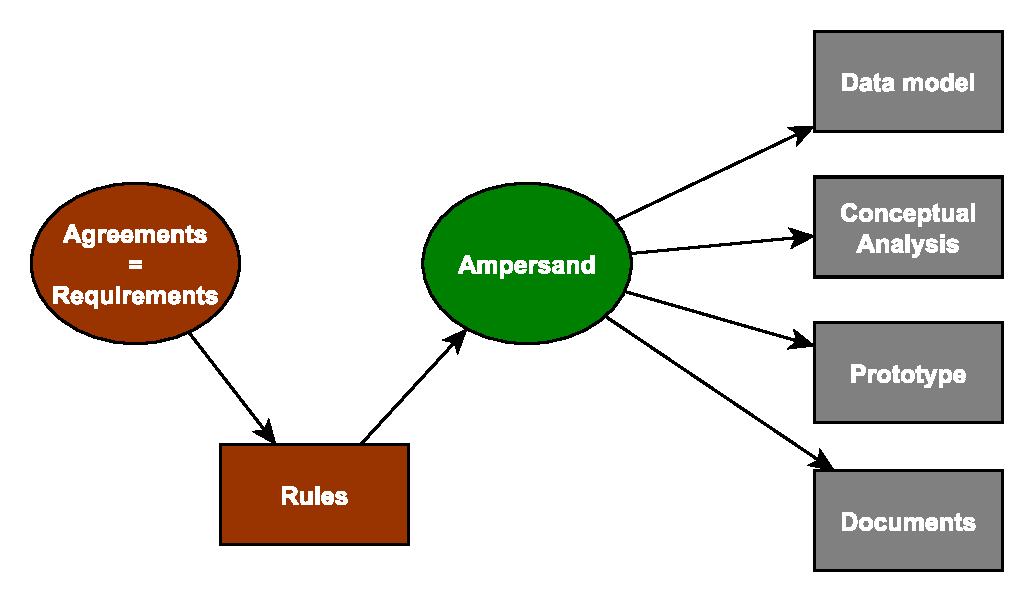
\includegraphics[width=0.7\textwidth]{Figures/Generation}
	\caption[Generated artifacts]{Ampersand generates several artifacts based on the business rules (source: \cite{ampersand-approach})}
	\label{fig:generation}
\end{figure}
%

The Ampersand project is used in several environments, by different user groups.
In a research context, the Ampersand project is part of the research on the use of business rules for software design.
In an educational context, it is also used as the main tool in the course `Rule Based Design' from the Open University of the Netherlands.
Finally, the compiler is used in business environments to design and develop real world business software.

% !TEX root = ../Thesis.tex

\subsection{High-level architecture}
\label{subsec:architecture}
The compiler developed for the Ampersand research project runs in several steps, hence the Ampersand compiler is also divided in several subcomponents:
\dict{P-structure}{The parse-tree generated by the Ampersand parser, used as input for the type checker}%
\dict{A-structure}{The ADL code generated by the Ampersand type checker, used as input for the calculator component}%
\dict{ADL-structure}{See A-structure}%
\dict{F-structure}{The functional structure generated by the Ampersand calculator, used as input for the different output modules}%
\begin{itemize}
	\item \textbf{Parser}: This component receives the ADL code as input, and parses that code into a parse-tree (also known as P-structure).
	\item \textbf{Type checker}: The Ampersand type checker receives a P-structure as input and converts it into a relational algebra format, suitable for manipulation (also known as A-structure or ADL-structure).
		 The semantics of ampersand are expressed in terms of the A-structure.
	\item \textbf{Calc}: The Calc component receives an A-structure as input, and manipulates it according to the research rules, generating the functional structure (also known as F-structure).
		The F-structure contains all design artifacts needed to write a specification and generate the output.
	\item \textbf{Output components}: All design artifacts present in the F-structure are ready to be rendered.
		Several components use this data structure to generate the wished output.
		The output components currently implemented (and their output formats) are the following: 
		\begin{itemize}
			\item Atlas (HTML interface);
			\item Revert (Haskell source);
			\item Query (prototype generation);
			\item Documentation Generator (Pandoc structure).
		\end{itemize}
\end{itemize}

% !TEX root = ../Documentation.tex

\subsection{Parser (R-M)}
\label{subsec:design-parser}
The mainstream design of the new parser has not changed much.
Basically, each EBNF rule receives its own parser function.
Thanks to the combinator operators, each parsing function also looks very similar to its corresponding EBNF.

The applicative interface is consistently used.
By changing details of the implementation, e.g. the order of the fields in the parse tree, we have made many of the `rebuild' functions unnecessary.
For some parsers the amount of changes necessary in order to remove supporting functions was too large or even impossible with the current parse tree.

Note that in parts of the parser, the function syntax has substituted the record syntax for creating data objects.
This was done only when the code readability could be improved by doing so.

\subsubsection{Parsec}
\label{subsec:design-parsing-lib}
As mentioned earlier, and described in research context document \citenac{parsing}, the new Ampersand parser has been rebuilt with another parsing library, namely Parsec.
However, for the Ampersand developers, the source code of the parser will still look very familiar, thanks to the applicative interface.
For developers, the main differences between Parsec and the uulib are:
\begin{itemize}
  \item Parsec does not backtrack by default.
    In order to enable backtracking, the \texttt{try} function must be used.
    This is described in \autoref{subsec:backtracking}.
  \item Parsec does not try to solve parsing errors.
    The parser stops immediately after the first issue.
    See also the error analysis in \autoref{subsec:design-errors}.
  \item Error messages are customizable by using the \texttt{<?>} operator.
    This is also suggested in \autoref{subsec:design-next-steps}.
  \item Some combinators have a different name, e.g. one must use \texttt{option} instead of \texttt{opt}.
    Assuming the documentation found on Hackage is clear and sufficient, interface differences are not documented here.
\end{itemize}

\subsubsection{Backtracking}
\label{subsec:backtracking}
In order to explain the differences on backtracking behavior between the uulib and Parsec, we quote here Doaitse Swierstra, the author of the uulib \citenac{swierstra-parsec}:
\begin{quote}
\textsl{To understand the subtleties it is important to understand the differences between the try construct in Haskell and the non-greedy parsing strategy used in uu-parsinglib. Effectively the latter is a try which just looks ahead one symbol. In that respect it is less powerful than the try construct from Parsec, in which you specify that a specific construct has to be present completely. And then there is the underlying different overall strategy. Parsec uses a back-tracking strategy with explicit tries to commit, whereas uu-parsinglib uses a breadth-first strategy with an occasional single symbol look-ahead.}
\end{quote}
%
We can therefore conclude that the try-statements in Parsec are undesirable.
However, they are necessary when the grammar is ambiguous.
In this section we explain why each of the remaining try statements are necessary, and how these issues can be resolved:
\begin{description}
  \item[Classify]
    This ambiguity in the grammar arises from the \texttt{Classify} and \texttt{GenDef} productions:
    \begin{quote}
        \texttt{Classify ::= `CLASSIFY' ConceptRef `IS' Cterm}\\
        \texttt{GenDef ::= (`CLASSIFY' | `SPEC') ConceptRef `ISA' ConceptRef}
    \end{quote}
    When the parser encounters \texttt{`CLASSIFY'}, it cannot define whether it found a \texttt{Classify} or a \texttt{GenDef} production.
    Therefore, the parser must consume the keyword and a \texttt{ConceptRef} before consuming either \texttt{`IS'} or \texttt{`ISA'} and determining which production is applicable.
    
    In order to solve this issue, one must choose a different keyword or symbol for each of the productions.
    Another option would be to merge the two statements in the same parser.
    We did not merge the productions because that would make the parser less maintainable.
  
  \item[Role]
    This ambiguity in the grammar arises from the \texttt{RoleRelation} and \texttt{RoleRule} productions:
    \begin{quote}
        \texttt{RoleRelation ::= `ROLE' RoleList `EDITS' NamedRelList}\\
        \texttt{RoleRule ::= `ROLE' RoleList `MAINTAINS' ADLidList}
    \end{quote}
    When the parser encounters \texttt{`ROLE'}, it cannot define whether it is a \texttt{RoleRelation} or a \texttt{RoleRule} production.
    Therefore, the parser must consume the keyword and a \texttt{RoleList} (which may be long) before consuming either \texttt{`MAINTAINS'} or \texttt{`EDITS'} and determining which production is applicable.
    
    In order to solve this issue, one must choose a different keyword for each of the productions, merge the two options to have the same representation in the parse tree, or refactor the parser so that the two options are parsed together.
    We did not merge the productions because that would make the parser less maintainable.
  
  \item[View]
    This ambiguity in the grammar arises from the \texttt{FancyViewDef} and \texttt{ViewDefLegacy} productions:
    \begin{quote}
        \texttt{FancyViewDef ::= `VIEW' Label ConceptOneRefPos `DEFAULT'? `\{' ViewObjList `\}' HtmlView? `ENDVIEW'}\\
        \texttt{ViewDefLegacy ::= (`VIEW' | `KEY') LabelProps ConceptOneRefPos `(' ViewSegmentList `)' }
    \end{quote}
    When the parser encounters \texttt{`VIEW'}, it cannot define whether it found a \texttt{FancyViewDef} or a \texttt{ViewDefLegacy} production.
    In this case, defining which construction is applicable is even more complicated.
    This decision must, in the worst case, be delayed until the parser encounters a \texttt{`\{'} or \texttt{'('}.
    That's because the productions \texttt{Label} and \texttt{LabelProps} are not disjoint, and \texttt{`DEFAULT'} is optional.
    
    In order to solve this issue, we advise to merge or drop the legacy statement.
    
  \item[Multiplicity]
    This ambiguity in the grammar arises from the \texttt{Mult} production:
    \begin{quote}
        \texttt{Mult ::= (`0' | `1') `..' (`1' | `*') | `*' | `1'}
    \end{quote}
    When the parser encounters \texttt{`1'}, it cannot define whether it found the first or the last production.
    The parser must therefore read the next token before choosing the right option.
    
    In order to solve this issue, we advise to refactor the grammar (and the parser) to have the following production:
    \begin{quote}
        \texttt{Mult ::= `0' `..' (`1' | `*') | `1'(`..' (`1' | `*'))? | `*'}
    \end{quote}
    %
    We did not refactor the code in this manner because the \texttt{pMult} parser does more than only parsing: it also changes the representation of the found constructions before creating the parse tree.
  
  \item[Labels and Terms]
    In the productions \texttt{Att} and \texttt{RuleDef}, we see very similar ambiguities:
    \begin{quote}
        \texttt{Att ::= LabelProps? Term}\\
        \texttt{RuleDef ::= `RULE' Label? Rule Meaning* Message* Violation?}
    \end{quote}
    Wherein:
    \begin{quote}
        \texttt{Label ::= ADLid ':'}\\
        \texttt{LabelProps ::= ADLid (`{' ADLidListList `}')? `:'}\\
        \texttt{Rule ::= Term ('=' Term | '|-' Term)?}
    \end{quote}
    And one of the possible productions of \texttt{Term} is:
    \begin{quote}
        \texttt{Term ::= Trm2 ::= Trm3 ::= Trm4 ::= Trm5 ::= Trm6 ::= RelationRef ::= NamedRel ::= Varid Sign?}
    \end{quote}
    While:
    \begin{quote}
        \texttt{ADLid ::= Varid | Conid | String}
    \end{quote}
    
    What happens here is that when the parser encounters a \texttt{Varid}, it cannot define whether it is part of the (optional) \texttt{Label} production or if no \texttt{Label} was given and the \texttt{Varid} is part of a \texttt{Term}/\texttt{NamedRel} production.
    
    Due to the quite complex grammar for the \texttt{Term} production, this issue may severely impact the parser's performance.
    This is probably the most harmful of the ambiguities mentioned.
    However, it can only be solved by adding a symbol before the \texttt{Term} production (e.g. making the `:' non-optional).
\end{description}
%
Please note that in order to have proper backtracking with correct error messages, Parsec may require two try-statements \citenac{try-harmful}.

% !TEX root = ../Thesis.tex

\subsection{Other objectives}
While designing and implementing the new Ampersand parser, the following objectives were also important:
\begin{itemize}
  \item \textbf{Integration}: The new parser must interface with the remaining Ampersand modules.
    It must thus be implemented in Haskell.
  \item \textbf{Libraries}: Since different implementation options are available, it was important to choose the most suitable Haskell parsing framework.
  \item \textbf{Maintainability}: Well-written and maintainable code is a must for the Ampersand project, since it is an open-source project.
    The maintainability must be either maintained or improved; otherwise the parser is not to be taken into production.
  \item \textbf{Tests}: Testing the parser well was a task for this project.
    The suggestion is to use testing tools to improve the process, e.g. QuickCheck.
  \item \textbf{Pretty-printing}: This is important in order to test the parser.
\dict{HPC}{Haskell Program Coverage}%
\dict{Haddock}{Software documentation generator for the Haskell programming language}%
\dict{HLint}{Statical analysis software that suggests maintainability improvements}%
  \item \textbf{Tools}: Within the Haskell community, several tools are popular to verify code quality and generate documentation, e.g. HPC, Haddock and HLint.
  \item \textbf{Fixed syntax}: The new parser must process the same inputs as the previous parser.
  \item \textbf{Fixed parse tree}: The new parser must produce the same outputs as the previous parser.
    Any further changes must be applied to the rest of the Ampersand system.
\end{itemize}

During the project, some additional requirements have been identified:
\begin{itemize}
  \item \textbf{Git/GitHub}: The changed software had to be integrated into the GitHub Ampersand project.
    The development itself happened in a separate branch of a separate fork, so that deliveries could be merged in a smooth way.
    This was an especially hard requirement for us, since we had no experience with Git.
  \item \textbf{Cabal}: The building system for Haskell had to be maintained as the building platform.
  \item \textbf{EBNF}: The syntax of the Ampersand grammar was specified in EBNF notation but was not up-to-date.
    Any changes to the syntax had to be documented according with this notation.
    One option was to add the EBNF as comment in the source code in order to make clear that the complete grammar is implemented correctly.
\end{itemize}

On top of the project goals, we also wanted to help the university and other students with our results.
Finally, building up knowledge was also important for us (i.e. functional programming, Haskell, compilers, parsers, LaTeX, Ampersand, business rules and research in general).


\newpage
% !TEX root = ../Thesis.tex

% individueel verslag onderzoek deeldomein en bijhorende technieken, plusminus 5 pagina's
% details van domein en technieken in relatie met het onderzoeksproject
% academische verantwoording gemaakte keuzen

\subsection{The Ampersand Approach (M)}
\label{domain:approach}
\lipsum[1]

\newpage
\documentclass[a4paper,12pt,abstracton,titlepage]{scrartcl}
\usepackage{scrpage2}
\usepackage[utf8]{inputenc}
\usepackage[T1]{fontenc}
\usepackage[top=2.5cm, bottom=2.5cm, left=2cm, right=2cm]{geometry}
\usepackage[affil-it]{authblk}
\usepackage{lipsum}
\usepackage{url}
\usepackage[hidelinks]{hyperref}
\usepackage{graphicx}
\usepackage[table,xcdraw]{xcolor}
\usepackage{longtable}
\usepackage{multicol}

%citations
\usepackage{multibib}
\newcites{ac}{Academic references}
\newcites{nac}{Informal references}

% code for generating glossary, from http://tex.stackexchange.com/a/5837/59718
\usepackage[acronym,toc]{glossaries}
\usepackage{glossary-mcols}
\newcommand{\dict}[2]{%
  \newglossaryentry{#1}{name=#1,description={#2}}%
  \glslink{#1}{}%
}
\makeglossaries

% Here we set up the header, meta-information and front matter
%\date{December 17, 2014}      %// Today's date will appear when this is commented out.
\newcommand{\version}{0.3}

% title page
\author{Daniel S. C. Schiavini}
\affil{Open Universiteit Nederland, faculteit Informatica \\
	T61327 - Afstudeerproject bachelor informatica}
\title{Haskell parsing libraries \&\\ user-friendly error messages}
\subtitle{Useful feedback in the Ampersand parser\\
	~\\
	Phase 3a: Domain \& Techniques}
\publishers{Version \version}

% header
\pagestyle{scrheadings}
\setheadsepline{0.2pt}
\clearscrheadings
\automark[section]{chapter}
\ihead{Daniel S.C. Schiavini}
\ohead{Parsing libraries \& error messages}
\cfoot{\pagemark}

% URL's
\renewcommand*{\UrlFont}{\footnotesize\ttfamily}

% hyphenation
\hyphenation{
	gua-ran-tee
	pro-duct
	cor-res-pon-ding
	me-cha-nism
	know-ledge
	de-ve-lo-pers
	do-cu-men-ta-tion
	sa-tis-fac-tion
	Schi-a-vi-ni
	Ba-ert-so-en}

% Now the document starts
\begin{document}
\maketitle
\newpage

\tableofcontents
%\listoffigures
%\listoftables
\clearpage

% !TEX root = ../Documentation.tex
\section{Introduction}
\subsection{Identification}
This document contains the domain \& techniques analysis of the project `Useful feedback in the Ampersand parser'.
The document is the milestone product of the project phase 3a for Daniel S.C. Schiavini, as specified in the project planning \citenac{plan}.

This document is part of the graduation project of the computer science bachelor at the Open Universiteit Nederland.
The project `Useful feedback in the Ampersand parser' is executed in collaboration with Maarten Baertsoen, with support of the supervisor Dr. Bastiaan Heeren and examiner Prof.dr. Marko C.J.D. van Eekelen.
The assignment is given by Prof.dr. Stef Joosten, who researches how to further automate the design of business processes and information systems by the development of the Ampersand project.

Ampersand is an approach for the use of business rules to define the business processes.
Users describe the business rules in a formal language (ADL), and Ampersand compiles those rules into functional specification, documentation and working software
prototypes.
The main objective of this project is to improve the feedback and maintainability of the Ampersand parser.
See \citenac{plan} for more details on the project.

\subsection{Goals}
\lipsum[3]

\subsection{Document overview}
\lipsum[4]
% !TEX root = ../Parsing.tex

\section{Haskell parsing libraries}
\label{sec:libraries}

\subsection{Parsing remarks}
\dict{Lexical analysis}{Separating text into tokens}%
\dict{Lexer}{Software that does the lexical analysis}%
\dict{Alex}{Lexer included in the Haskell Platform}%
Parsing is sometimes divided into two stages: lexical analysis (separating the source text into tokens) and parsing itself (constructing a parse tree).
Tools such as the ones analyzed here can perform both lexical analysis and parsing.
However, sometimes the tools can be more efficient when supported by a separate Lexer (e.g. Alex).

Grammars associated with a formal language are described as a set of production rules.
Since these rules are formally defined, a series of mathematical constructions can be used to manipulate and describe the grammar.

\dict{ADL}{Ampersand Definition Language}%
\dict{BNF}{Backus-Naur Form, a meta-syntax notation for expressing context-free grammars}%
\dict{EBNF}{Extended Backus-Naur Form, an extension on BNF}%
The Ampersand Definition Language (ADL) is specified in a grammar in the Extended Backus-Naur Form (EBNF).
Even though it is known that the grammar is not up to date, this article assumes the updated version will not fundamentally be different than the specified grammar.

\subsection{Generators vs. combinators}
\dict{DSL}{Domain specific language}%
Generally, there are two options for implementing a parser:
The first option is to implement the parser in the language of choice, i.e. Haskell for this project.
Another possibility is to use a domain-specific-language (DSL) to describe the grammar, and let a separate software generate the actual parsing code.
The two approaches and their advantages and disadvantages are described in this section.

\subsubsection{Parsing libraries}
When programmers go down the path of building a parser directly in Haskell, building up a set of functions that support parsing is a natural consequence.
Although it's possible to build these functions for each and every project \cite{monadic-parsing}, using a premade library has several advantages, e.g. reduced effort, increased functionality, optimized performance and better documentation.
The extra effort to learn the library is paid off by these advantages.
In Haskell this is mostly done by providing monadic combinators to hold up extra information about the parsing state, and results in very elegant solutions \cite{monadic-parsing}.

The parsers built in Haskell are mostly recursive descent parsers, wherein the parser runs top-down from a set of recursive calls.
The program structure is then closely related to the production rules, supporting the readability of the program structure.

These parsers analyze the input text from \underline{L}eft to right and choose the \underline{L}eftmost derivation in the grammar.
Such parsers are called therefore LL parsers.

~\\
However, there are limitations related to recursive descent parsers.
For instance, a common kind of production rule is a left recursive one, e.g. \texttt{term $\rightarrow$ term `$+$' term $|$ digit}.
In this case, the first thing the parser would do is call itself, resulting in an infinite loop.
Gladly, left recursive grammars can be converted into right recursive ones \cite{remove-left}.

Therefore, LL parsers may require exponential time to run and are not able to guarantee termination.
In order to guarantee termination and linear execution time, a recursive descent parser must be able to recognize which production rule to use by reading only limited amount of tokens.
This is only possible for the class of unambiguous grammars without left recursion.

~\\
\dict{LL(k)-grammar}{A grammar that can be parsed by an LL($k$)-parser}%
\dict{LL(k)-parser}{Top-down parser that parses from left to right, performing the leftmost derivation with a maximum $k$-tokens of look-ahead}%
The EBNF for the ADL-language is not ambiguous and has no left recursion.
This grammar can therefore be called an LL($k$)-grammar, for which an LL($k$)-parser can be created.
The $k$ between the parenthesis means that this parser needs a maximum of $k$ tokens of look-ahead in order to choose a production rule.

\subsubsection{Parser generators}
As mentioned, another approach for building a parser is to specify the software's grammar in a specific notation and use a parser generator to create the actual parser source code.
In the domain of context-free grammars, a widely used grammar notation is the Backus-Naur Form (BNF).

\dict{Happy Parser Generator}{Parser generator system for Haskell. \url{https://www.haskell.org/happy/}}%
This research is focused in the Happy parser generator, which is part of the Haskell Platform since 2001.
Happy inputs a file containing an annotated BNF specification of a grammar and produces a Haskell module with a parser for that grammar.
Since it is possible to convert EBNF to BNF \cite{convert-ebnf,bnf-ebnf}, a Happy parser should not involve a lot of effort.
It is important to know, however, that besides converting the EBNF to BNF, the annotation still requires effort and knowledge acquisition.

\dict{LR parser}{Top-down parser that parses from left to right, performing the rightmost derivation}%
A parser generator is able to execute statical analysis on the input grammar.
Besides, they are often able to recognize more complicated grammars by running \underline{L}eft-to-right, and picking the \underline{R}ightmost derivation, being called therefore an LR parser.

\dict{LALR parser}{LR parser with look-ahead}%
An LR parser with \underline{L}ook-\underline{A}head is called an LALR parser.
By performing the rightmost derivation of the production rules, an LALR parser is able to recognize more complex grammars.
However, its workings are quite unintuitive, and understanding such parsers can be very hard.
That's exactly why LALR parsers are usually generated instead of built by hand.

Since understanding LALR parsers is hard, the syntax errors caused by incorrect input may be much harder to pinpoint and understand.
The errors generated by LALR parsers are often not in high-level terms that the end users can understand.

\dict{GHC}{Glasgow Haskell Compiler}%
\dict{Hugs}{Haskell Compiler}%
\dict{YACC}{Yet Another Compiler Compiler}%
\dict{Hellium}{Haskell Compiler}%
\dict{GCC}{Gnu Compiler Collection}%
Haskell compilers GHC and Hugs are both built with LALR generated parsers: Hugs is written in YACC and GHC is built with Happy \cite{hugs-parser,ghc-parser}.
Later on, the Helium compiler was created for classroom-use because the mentioned Haskell compilers were not user friendly \cite{helium-parser}.
Other examples are the GCC compilers for C and C++, that started as LALR generated compilers and were remade to be recursive-descent parsers \cite{gcc-c-parser,gcc-cpp-parser}.

Although it's harder to understand its workings, the resulting source code for the generators is simpler and easier to maintain, as can be seen in \cite{parser-examples}.

\subsubsection{Conclusion}
In the context of the new Ampersand parser, some advantages of building the parser in Haskell instead of using a generator, are:
\begin{description}
	\item[Flexibility] The programming language gives much more flexibility in coping with context-sensitive grammars.
	\item[Building] The process is simpler since it is unnecessary to run a separate program to generate the parser.
	\item[Language] Both the customer and the project members feel more comfortable working in Haskell then in an unknown DSL.
	\item[Errors] The main objective of the project is giving useful feedback in the new Ampersand parser, and this seems much easier to achieve with a handwritten parser.
\end{description}

\noindent
On the other hand, the advantages of using a parser generator, instead of handwriting the code, are:
\begin{description}
	\item[Optimizations] Because the parser is generated on-the-fly, the generator can apply optimizations that would otherwise be hard to implement.
	\item[Performance] Bottom-up parsers are much more efficient because they are able to pack the code into state machines.
		This is even more valid when many parsing alternatives are available.
	\item[Static analysis] The generator is able to do a lot more static analysis, while a library is only executed during the run-time.
    E.g. programmers will only know of left recursions and non-terminations by testing the parser.
	\item[Documentation] Since the DSL is basically annotated BNF, keeping the syntax diagrams up to date is much easier.
\end{description}

\noindent
From the above advantages and disadvantages, it is clear that no universal truth exists in these matters.
Although it is a difficult choice, the error messages are indeed the most important project target, so writing the parser by hand is the advised option.
This choice also means that it keeps on being a task of the developers to update the documentation, e.g. the syntax diagrams that are currently not up-to-date.

\subsection{Combinator libraries}
In the previous section, the choice to use a combinator library has been taken.
In this section, two libraries will be compared: the Utrecht University parser combinator library (uu-parsinglib) and Parsec.
Other libraries (e.g. Attoparsec, Polyparse) are out of the scope of this research.

\subsection{Utrecht University Parsing Library}
\dict{uu-parsinglib}{Haskell parsing library from the Utrecht University. \url{http://foswiki.cs.uu.nl/foswiki/HUT/ParserCombinators}}%
The uu-parsinglib is a combinator library created by Doaitse Swierstra in the Utrecht University.
This library is used in many mature projects.
The current Ampersand parser is also built with the previous version of the uu-parsinglib.
The new version has several improvements, mainly in performance \cite{benchmark}.
It currently has more than 4 thousand downloads in the Hackage package manager.

The documentation is mainly in Haddock format and in a paper from 2009 \cite{uu-doc}.
The implementation is open source.
The new version of the uu-parsinglib provides combinators that include error correction and a monadic interface.
Errors are recognized and corrected automatically if the programmers want so, but the reporting is customizable.
It also supports grammars that are not context-free and even ambiguous grammars (provided the user accepts exponential run-time).

Finally, the uu-parsinglib runs online, i.e. it returns parts of the parsing three as soon as they are ready.
This gives programmers the ability to do lazy parsing.

\subsection{Parsec}
\dict{Parsec}{Haskell monadic parsing combinator library written by Daan Leijen. \url{https://www.haskell.org/haskellwiki/Parsec}}%
Parsec is a monadic parsing combinator library created by Daan Leijen, while also working at the Utrecht University.
It seems to be the most popular combinator library in the Haskell community, with more than 200 thousand downloads in the Hackage package manager.

Parsec is designed to be simple, safe and well documented industrial parser library.
Besides, there has also been some work done on the performance and error messages.
The documentation of Parsec and its documentation tends to be better than that of the uu-parsinglib because of a larger user base.

%todo: this section is very empty
%todo: https://www.haskell.org/haskellwiki/Parsec
%todo: http://stackoverflow.com/questions/19208231/attoparsec-or-parsec-in-haskell/19213247#19213247

\subsection{Monadic vs. arrow interfaces}
Monads allow sequences and state to be saved during the parsing, and had become the most common way of building Haskell parsers.
Until, in a paper from Swierstra \cite{error-correcting}, a parsing library was published with an alternative interface.
Hughes presented this alternative as a generalization of monads, calling it `arrows' \cite{monad-arrows}.

Arrows are less convenient than monads but are much widely applicable \cite{monad-arrows}.
Monads would still be used for state passing and other constructions, but the continuations would be carried over to arrows.

Arrow-style parsers do not depend on the run-time values -- they are not dependent on the context.
This means that it is then possible to analyze and optimize the parser before executing it.
Swierstra goes so far to say that this works as a run-time parser generator \cite{error-correcting}.
On the other hand, the lack of context means that only context-free languages can be implemented this way \cite{parsec}.

The uu-parsinglib allows both monadic and arrow-style parsing, while Parsec only has a monadic interface.
In the arrow-style interface, the uu-parsinglib also adds error correction:
After detecting an error, the library will correct it by adding or deleting tokens.
It then generates an appropriate error message and continues with the rest of the program.
By using this interface, the parsing will thus always succeed.

%todo: http://worldbusiness.org/wp-content/uploads/2012/10/arrows-and-idioms2.pdf
%todo: http://marc.info/?l=haskell-cafe&m=128039136131494

\subsection{Conclusion}
The following differences have been found between the two considered libraries:
\begin{description}
	\item[Documentation] The documentation of Parsec seems to be more extended and well-maintained.
		Several Parsec tutorials can be found on the internet (e.g. \cite{using-parsec}).
		On the other hand, the uu-parsinglib's documentation is mostly generated from code annotations.
	\item[Support] Since Parsec is much more used, online support can be more easily found.
		For example, the website Stack Overflow currently has 14 questions about the uu-parsinglib and 301 about Parsec.
	\item[Static checking] None of the libraries is able to do static checking.
		However, the uu-parsinglib has more possibilities of grammar analysis in its arrow-style interface.
	\item[Precedences] The Ampersand parser is currently built with the uu-parsinglib with great satisfaction.
		This both means that the library has enough features and that it is known by the other Ampersand developers.
	\item[Error reporting] No literature has been found with a comparison of the errors generated by the libraries.
		However, many publications affirm that the generated errors from both libraries are great \cite{helium-parser,benchmark,uu-doc,error-correcting,parsec}.
	\item[Error recovery] When a parsing error is found, a Parsec parser stops immediately.
		A parser built with uu-parsinglib, however, corrects the error and continues parsing.
		Error correction is good because the parser always succeeds.
		On the other hand, a big list of errors can also overwhelm the user \cite{heeren-error}.
		Finally, to perform the corrections, the parser needs to make assumptions based e.g. on statistics;
		these assumptions cannot always be correct.
	\item[Fine-tuning] According to the Helium development team, Parsec's possibilities for error fine-tuning are greater \cite{helium-parser}.
		However, to apply optimizations it is necessary to know the internal workings of the parser \cite{uu-doc}.
	\item[Backtracking] Parsec works with more traditional backtracking algorithms \cite{parsec} that can often lead to high space consumption \cite{uu-doc}.
		Backtracking must be manually activated, though.
	\item[Performance] The Parsec library seems to have better performance \cite{benchmark}, but the difference is small and is not expected to make a considerable difference in the small ADL scripts.
	\item[Try operator] In order to allow backtracking, Parsec code uses the try-function, which is considered harmful and can be easily misused \cite{try-harmful}.
		This keyword is totally unnecessary in the uu-parsinglib because it uses breadth-first lazy parsing \cite{uu-doc}.
		%todo: http://osdir.com/ml/haskell-cafe@haskell.org/2012-01/msg00566.html
	\item[Maintainability] No significant difference has been found in the maintainability of the two analyzed libraries.
		Note that the programmers working on Ampersand are already familiar with the uu-parsinglib.
		On the other hand, there is more support and documentation available for Parsec, so it can also be seen as more future-proof.
		The responsibility for the maintainability still lies on the hands of the programmers building the parser.
	\item[Origin] Both libraries are originated at the Utrecht University.
		In 2003, a Haskell compiler focused on user friendliness, Helium, was published from the same university.
		Knowing both libraries very well, the authors made the choice to use Parsec because of the possibilities of error customization \cite{helium-parser}.
\end{description}
%
Considering these differences, a deeper analysis of error messages is given in the next section.
The actual library choice is delayed until \autoref{sec:conclusion}.

% !TEX root = ../Thesis.tex

\subsection{Errors}
\label{analysis:errors}
%TODO: Bastiaan suggests we should try to use the definition of the error manifesto by Yang et al. (page 32 of his doctor)
In this section, we analyze the error messages given by the previous parser.
The results of this analysis are compared with the new parser in \autoref{tests:errors}.

\subsubsection{Error message qualification}
The user friendliness and correctness of an error message is a subjective topic and therefore we need to start with a definition to objectively judge the quality of an error message.
After analyzing the current Ampersand parser error messages, we identified the following objective aspects of an Ampersand parser error message:
%
\begin{description}
	\item [Position]
	Each error messages reports the correct position (file, line number and column) of where the user committed the error.
	\item [Accuracy]
	The accuracy of an error message is measured based upon the following characteristics:
	\begin{enumerate}
		\item	\textbf{\small How does the provided error description outline the discovered error:}
				Providing the user with a good description of the encountered syntax issue will support a fast error resolution.
				When the issue is vaguely described without pinpointing the exact issue, the error resolution will be time consuming.
		\item	\textbf{\small Pinpointing the correct error}:
				An error can lead to multiple subsequent issues.
				These issues are, however, irrelevant for the user and the Ampersand parser should provide the exact origin of the issues.
		\item	\textbf{\small Quality of the hint:}
			The message can provide a hint for a solution together with the error message to support the user with the error resolution.
	\end {enumerate}
    \item[Conciseness]
	Providing a good error description is one thing, but this one message can be hidden between several other error messages that result from the initial error.
	It is unlikely that users will easily find the exact originating issue in their source file when they are overwhelmed with a multitude of error messages. % using plural to avoid repeating his/her
\end {description}
%
Based on these objective properties to judge the quality of the parsing errors, we defined the following criteria to distinguish between good, bad and average (but acceptable) error messages:
%
%TODO: Bastiaan doesn't think there's a main originating error. See his review in page 15.
\begin{description}
	\item [Bad error message] A message is considered to be bad if one of the criteria below is fulfilled:
		\begin{description}
			\item [Position]
			The position has a deviation of more than one line or ten column positions from where the actual error is made.
			\item [Accuracy]~
				\begin{itemize}
					\item 	The provided error description is useless for the user to determine the actual error.
					\item 	The provided error description is not appointing the main, originating error without any correlation towards this main error.
				\end {itemize}
			\item[Conciseness]
			More than distinct three errors are mentioned by the Ampersand parser.
		\end {description}
	\item [Acceptable error message] A message is considered to be of average, but acceptable, quality if one of the criteria below is fulfilled:
		\begin{description}
			\item [Position]
			The position has a deviation between five and ten column positions from where the actual error is made.
			\item [Accuracy]~
				\begin{itemize}
					\item 	The provided error description is not an exact description of the error, but provides 6useful information to discover the actual issue.
					\item 	The provided error description is not appointing the main originating error, but the link to the actual error can be discovered based on the provided information.
					\item 	The provided hint is incorrect.
				\end {itemize}
			\item[Conciseness]
			two or three errors are mentioned by the Ampersand parser.
		\end {description}
		
	\item [Good error message] Any error message that is not bad nor acceptable is good.
\end {description}

\subsubsection{Gathering process}

To gather the necessary input for the as-is analysis, an exhaustive list of all possible error messages is created.
This as-is analysis will be used as a reference base to verify the implementation of the new error mechanism with Parsec.
The errors are invoked by simulating all possible syntax errors that will invoke an error within the Ampersand parser.
Each syntax statement is therefore manipulated, introducing one specific error per time, and the resulting error message is then recorded together with the actual erroneous statement.
The exact same statements are afterwards pushed through the new parser, making it possible to make a quantitative `before and after' analysis.
Special attention is given to avoid redundant errors that could influence the quantitative analysis. 
An example of such an redundant error is the use of a capital letter in defining a specific reference. 
Although these references are used in several syntax statements, there is only one procedure in the parser to check all references starting with a capital letter.
An improvement in the error message of this check may only be taken into account one time.

\subsubsection{Results}
Based on our error message qualification definition, \autoref{tab:error-messages-analysis} visualizes the results of the as-is analysis.
This analysis clearly confirms the statement that the quality of the error messages is of low quality and that there is a lot of room for improvement.

% Please add the following required packages to your document preamble:
% \usepackage[table,xcdraw]{xcolor}
% If you use beamer only pass "xcolor=table" option, i.e. \documentclass[xcolor=table]{beamer}
\begin{table}[h]
  \centering
	\begin{tabular}{llrlr}
    Error quality  & \multicolumn{2}{c}{Previous parser}     \\
		Good           & 19          & 22,35\%         \\
		Acceptable        & 48          & 56,47\%       \\
		Bad            & 18          & 21,18\%           \\
		\rowcolor[HTML]{BBBBBB}
		\textbf{Total} & \textbf{85} & \textbf{100,00\%} 
	\end{tabular}
  \caption{Error message as-is analysis results}
  \label{tab:error-messages-analysis}
\end{table}

% !TEX root = ../Parsing.tex

\section{Conclusion}
\label{sec:conclusion}
In \autoref{sec:libraries}, the advice was given to use a combinator library for the new parser of Ampersand.
The main reason to avoid the parser generators is that it is hard to generate useful feedback.
Then, in \autoref{sec:errors}, it was made even more clear that besides generating good messages, those messages should also be customizable.

Therefore, the advice of this research is to use the combinator library that offers the highest level of customization in error messages, Parsec.
Although the uu-parsinglib seems to also be a very good choice, the experiences from the Helium compiler \citeac{helium-parser} should be also considered.
Besides, the Parsec library offers better support.

A list of important consideration points has also been collected through the literature and can be found in \autoref{sec:errors}, more specifically \ref{subsec:errors-ampersand}.

\part*{Appendices}
\addcontentsline{toc}{part}{Appendices}
\appendix
% !TEX root = ../Parsing.tex

\small
\printglossary[style=mcolindex,title=Glossary]
\label{sec:glossary}

% !TEX root = ../Parsing.tex
\addcontentsline{toc}{section}{References}
\label{sec:bibliography}

\begin{thebibliography}{99}

\bibitem{plan}
	Planning for the project `Useful feedback in the Ampersand parser'\\
	Maarten Baertsoen and Daniel S. C. Schiavini\\
	Version 2.0 -- November 29, 2014\\
	\url{http://git.io/NeHuLg}

\bibitem{heeren-error}
	Top Quality Type Error Messages\\
	Bastiaan Heeren\\
	ISBN 90-393-4005-6, September 20, 2005\\
	\url{http://www.open.ou.nl/bhr/phdthesis}

\bibitem{monadic-parsing}
	Functional pearls -- Monadic Parsing in Haskell\\
	Graham Hutton (University of Nottingham) and Erik Meijer (University of Utrecht)\\
	\url{http://www.cs.nott.ac.uk/~gmh/monparsing.pdf}

\bibitem{convert-ebnf}
	 From EBNF to BNF \\
	 Christoph Zenger\\
	 June 4, 2000\\
	 \url{http://lampwww.epfl.ch/teaching/archive/compilation-ssc/2000/part4/parsing/node3.html}

\bibitem{bnf-ebnf}
	BNF and EBNF: What are they and how do they work?\\
	Lars Marius Garshol\\
	August 22, 2008\\
	\url{http://www.garshol.priv.no/download/text/bnf.html}

\bibitem{parser-examples}
	Haskell Parser Examples\\
	Geoff Hulette\\
	August 22, 2014\\
	\url{https://github.com/ghulette/haskell-parser-examples}

\bibitem{hugs-parser}
	Source code of the Hugs parser\\
	March 25, 2007\\
	\url{https://github.com/fuzxxl/Hugs/blob/master/src/parser.y}

\bibitem{ghc-parser}
	GHC: The Parser\\
	December 1, 2014\\
	\url{https://ghc.haskell.org/trac/ghc/wiki/Commentary/Compiler/Parser}
	%\url{https://ghc.haskell.org/trac/ghc/browser/ghc/compiler/parser/Parser.y}
	%https://www.haskell.org/pipermail/haskell-cafe/2013-August/109557.html

\bibitem{helium-parser}
	Helium, for Learning Haskell\\
	Bastiaan Heeren, Daan Leijen, Arjan van IJzendoorn\\
	Utrecht University\\
	\url{http://www.open.ou.nl/bhr/heeren-helium.pdf}
	
\bibitem{gcc-c-parser}
	GCC 4.1 Release Series Changes, New Features, and Fixes\\
	\url{https://gcc.gnu.org/gcc-3.4/changes.html}

\bibitem{gcc-cpp-parser}
	GCC 3.4 Release Series Changes, New Features, and Fixes\\
	\url{https://gcc.gnu.org/gcc-4.1/changes.html}
	
\end{thebibliography}

\end{document}
\newpage
\documentclass[a4paper,12pt,abstracton,titlepage]{scrartcl}
\usepackage{scrpage2}
\usepackage[utf8x]{inputenc}
\usepackage[T1]{fontenc}
\usepackage[top=2.5cm, bottom=2.5cm, left=2cm, right=2cm]{geometry}
\usepackage[affil-it]{authblk}
\usepackage{lipsum}
\usepackage{url}
\usepackage[hidelinks]{hyperref}
\usepackage{graphicx}
\usepackage[table,xcdraw]{xcolor}
\usepackage{longtable}
\usepackage{multicol}

%citations
\usepackage{multibib}
\newcites{ac}{Academic references}
\newcites{nac}{Informal references}

% code for generating glossary, from http://tex.stackexchange.com/a/5837/59718
\usepackage[acronym,toc]{glossaries}
\usepackage{glossary-mcols}
\newcommand{\dict}[2]{%
  \newglossaryentry{#1}{name=#1,description={#2}}%
  \glslink{#1}{}%
}
\makeglossaries

% Here we set up the header, meta-information and front matter
\date{June 11, 2015}      %// Today's date will appear when this is commented out.
\newcommand{\version}{1.0}

% title page
\author{Daniel S. C. Schiavini and Maarten Baertsoen}
\affil{Open Universiteit Nederland\\
    Faculteit Management, Science and Technology \\
	T61327 - Afstudeerproject bachelor informatica}
\title{Research Context}
\subtitle{Useful feedback in the Ampersand parser\\
	~\\
	Phase 3b}
\publishers{Version \version}

% header
\pagestyle{scrheadings}
\setheadsepline{0.2pt}
\clearscrheadings
\automark[section]{chapter}
\ihead{Daniel S.C. Schiavini and Maarten Baertsoen}
\ohead{Ampersand Parser: Research Context}
\cfoot{\pagemark}

% URL's
\renewcommand*{\UrlFont}{\footnotesize\ttfamily}

% Questions and answers
\newcommand{\question}[1]{\noindent\textbf{#1}\\}
\newcommand{\answer}[1]{#1\\}

% hyphenation
\hyphenation{
	gua-ran-tee
	pro-duct
	cor-res-pon-ding
	me-cha-nism
	know-ledge
	de-ve-lo-pers
	do-cu-men-ta-tion
	sa-tis-fac-tion
  sup-por-ting
	Schi-a-vi-ni
	Ba-ert-so-en}

% Now the document starts
\begin{document}
\maketitle
\newpage

\tableofcontents
%\listoffigures
%\listoftables
\clearpage

% !TEX root = ../Documentation.tex
\section{Introduction}
\subsection{Identification}
This document contains the domain \& techniques analysis of the project `Useful feedback in the Ampersand parser'.
The document is the milestone product of the project phase 3a for Daniel S.C. Schiavini, as specified in the project planning \citenac{plan}.

This document is part of the graduation project of the computer science bachelor at the Open Universiteit Nederland.
The project `Useful feedback in the Ampersand parser' is executed in collaboration with Maarten Baertsoen, with support of the supervisor Dr. Bastiaan Heeren and examiner Prof.dr. Marko C.J.D. van Eekelen.
The assignment is given by Prof.dr. Stef Joosten, who researches how to further automate the design of business processes and information systems by the development of the Ampersand project.

Ampersand is an approach for the use of business rules to define the business processes.
Users describe the business rules in a formal language (ADL), and Ampersand compiles those rules into functional specification, documentation and working software
prototypes.
The main objective of this project is to improve the feedback and maintainability of the Ampersand parser.
See \citenac{plan} for more details on the project.

\subsection{Goals}
\lipsum[3]

\subsection{Document overview}
\lipsum[4]
% !TEX root = ../ResearchContext.tex

\section{Short research}
\label{sec:research}
By investigating the requirements defined in the project planning \citenac{plan}, we identify here two contexts in which the new Ampersand parser is implemented.
First, we identify the Ampersand context, thus the research for the formal definition of business rules and the generation of documentation and software based  on it.
Second, we identify the parser context, thus the research for better user feedback in parsers.
In the following subsections each of the two contexts are described, including our findings during the literature research.

\subsection{Ampersand}
The Ampersand project has the ambition to offer a holistic methodology, including supporting tools, to support organizations during a software development project.
A new way of business requirements gathering, using natural language, is introduced by Ampersand.
We define the Ampersand approach by the Ampersand Methodology including the corresponding tools to create design artifacts and working software prototypes.

\subsubsection{Rule based design}

One of  the objectives of Ampersand is to bridge the gap between business analysts and system designers using natural language.
This objective is part of a general research context describing information systems based on business rules.

Kestutis Kapocius and Tomas Danikauskas \citeac{kapoc353} outline the use of an Output Driven Requirements Specification Method, ODRES, in combination with a Business Rules, BR, approach. 
In this approach, the BR approach formulates business rules in natural language using the Business Rules Solution, BRS, RuleSpeak model, Ronald Ross  \citeac{RuleSpeak}.
%TODO: good reference to add of RuleSpeak.
The Ampersand Language, describing the rules and syntax, can be seen as a formalization of the RuleSpeak guidelines and best practices.

\subsubsection{Ampersand target group context}
The Ampersand approach currently has 2 target groups: business analysts, in a commercial context, and students, in an educational context.

In the commercial context, the Ampersand users are typically business analysts who don't necessarily have programming experience.
The goal of these users is to specify, often complex, business rules in the most efficient way possible while still avoiding ambiguity.
To achieve their goals, the strictness of formal languages are a `necessary evil'.
Therefore, syntax errors can be very frustrating for the users.

Experiences within the Open Universiteit have shown that business analysts need roughly 100 hours to learn how to formalize business rules using Ampersand \citeac{joosten2007deriving}.
The learning costs can be thus quite high for organizations and students, and any improvement that can be made in the accessibility of Ampersand is welcome.

In the educational context, the Ampersand Users are students focusing on the domain of Rule Based Design. 
Within the course assignments, the students must check the completeness and consistency of their rule sets using Ampersand. 
 
Lex Wedemeijer \citeac{CSERC2013_Wedemijer} states that the instructional software must be powerful, yet basic.
The advanced features, offered to professional users, is not needed for students, moreover, the usage of a rich modeling features has a negative impact on the students learning curve.
The conclusion is made by Lex Wedemeijer that Ampersand may not be the perfect tool to support these student due to the richness of the language.
A more straightforward language, referred to as the Essential Language, is proposed, with clear and unambiguous notations, which is more suited to support students in the domain of Rule Based Design.

Providing a clearer error feedback in Ampersand does not lower the hurdle of the syntax richness, it is however a step in the good direction to better support the students. 
An interesting next step is the possibility to re-use the Ampersand vision and tools to support the easier to learn syntax of The Essential Language. 
To options to realize the re-use of Ampersand, is to simplify Ampersand towards the Essential Language or to implement a translator between both syntaxes.
Given the similarities between both languages, the translator seems the best approach, additional research is however needed to confirm this statement.

Andrei Lapets \citeac{lapets2009improving} concludes that user accessibility has not been a priority in the design of most formal verification systems.
He concludes that the syntax is often unfamiliar and/or introduces an entire new environment the user has to learn how to work with.
Finally, he points out that formal systems often offer a bottom-up structure that forces users to implement the complete set of assumptions in their research domain; this is made worse by the fact that usually few external libraries are available.

There are several measures that can be taken in order to improve the accessibility.
For example, the syntax should be familiar, simple and concrete \citeac{lapets2009improving}.
However, this project does not have any influence in the syntax.
The syntax of the ADL language is a given, so our influence is constrained to better user errors and development maintainability.

\dict{IDE}{Integrated development environment}
Pim Bos \citeac{bos2013bedrijfsregels} made a comparison between the tools for semantic web and Ampersand.
He concludes that the tools (e.g. script editors or an IDE) for supporting the development of Ampersand projects are lacking.
The fact that the ADL-compiler is currently the only feedback tool for users, stresses how important the feedback from the compiler is important.

Another issue named by Bos is the fact that the Ampersand user base is small.
A large user base is important for organizations using the tool, since they need to find specialists to implement and maintain the system.
It is also important for students and researchers, who may have difficulty finding peers to support and review their work.
Hopefully a better user feedback may also facilitate a larger user base.

The issues related with the lack of libraries and the bottom-up approach are named by both Lapets \citeac{lapets2009improving} and Bos \citeac{bos2013bedrijfsregels}.
To address this problem the institute Informatiegilde has been created \citeac{foutvrije-specificaties}.
This institute aims to organize an open-source repository of rules that can be used by anyone.

\subsection{Parsing errors}
%TODO: how can we integrate some info regarding the parser research context in regards to natural language processors, chatbots...
Although the new Ampersand parser has no influence on the research for better user feedback in parsers, it is important to identify this context because it is of great importance for the project.
Our literature research was focused on the error messages for parsers implemented in Haskell, and then mainly the LL($k$) parsers built with the Parsec library, which was chosen during our domain and technique research \citenac{parsing}.

Parsec has extensive error messages; giving position, unexpected input, expected productions and general user messages.
The error messages are given in terms of high-level grammar productions and can be localized for different (natural) languages \citeac{parsec-fast}.
Special care must be taken when using backtracking (the $try$-function) in the parsec library, as it may negatively influence the error messages generated \citeac{parsec}\citenac{try-harmful}.

Swierstra and Duponcheel \citeac{swierstra1996deterministic} describe how automatic error correction can be implemented.
This automatic error correction was used in the previous Ampersand parser.
However, the shortcomings of error correction have been described in our techniques research \cite{parsing} so this possibility is not used in the new Ampersand parser.












% !TEX root = ../ResearchContext.tex

\section{Expert consultation}
\label{sec:expert-consultation}
The following questions have been formulated during and after the literature research.
The questions have been asked to a researcher involved in the domain of Rule Based Design and the Semantic Web, namely Lloyd Rutledge.
Lloyd is currently an Assistant Professor at the Open Universiteit.
During the literature study, Lloyd already helped us finding interesting investigation topics and possible links to other research contexts during two alignment sessions.
The questions below are presented in the order they are listed below.
His answers are recorded literally after each of the questions, our own perception of the answers in relation to the research context are summarized in the conclusion, \autoref{sec:conclusion}.

~\\
\question{What do you use Ampersand for?}
\answer{
Students in our Masters course Rule-Based Design use Ampersand to implement business rules from case studies as a course assignment, which determines a large part of their course grade.
I also supervise several Masters Thesis students who perform their own research using Ampersand.
They often implement a case study in Ampersand to test hypotheses about how to establish business rules.
Our main current research theme is design patters for business rules.
We are starting a series of Masters Thesis research projects that propose rule design patterns and evaluate them in various case studies.
}

\question{What are the largest user complaints when using Ampersand?}
\answer{
Mostly complaints regard lack of documentation.
Inconsistencies between new versions of the software and the older software that exists is also a concern.
}

\question{Do you know whether users appreciate the error correction done by the previous parser?}
\answer{
No, I do not.
}

\question{Would better user feedback allow for a more efficient research on formal business rules?}
\answer{
I see no direct relation between user feedback and research.
It may have an indirect effect by making all work with Ampersand easier.
}

\question{Has the maintainability of the previous parser been an issue in your research?}
\answer{
I have had no complaints from Masters Thesis researchers, just as the course students have not complained to me about the parser.
It could be because the students are often business and management students, and thus the course may often be seen as a management theory course.
And then the course is secondly seen as the application of formal logic to business rules.
But on that level it is more a mathematical exercise than a computer project.
That there is software to process the rules into charts may be seen by many students as a secondary tool for helping establish the logic formalisms and the more strictly written business rules in natural language.

The research that I directly execute is more about the Semantic Web, its logic and its tools.
}
  
\question{How can a new Ampersand parser and better user feedback support the objectives of the Ampersand project?}
\answer{
By helping users more quickly write Ampersand scripts that function as expected and that deliver the desired insights.
}

\question{Is a better user feedback sufficient to optimize the learning path of students?
Or should a syntax simplification be considered for this target group?}
\answer{
There are too many aspects for optimizing learning paths to state that one tool would be sufficient.
Syntax simplification is another research area.
It has often been applied to business rules, both as non-computer and computer-processed syntaxes.
Our research's logical foundation is relation algebra, and so for us any simplified syntax would have to be equivalent to relation algebra.
Keywords may be easier in the beginning to work with than logical symbols.
But in the long run it is the form and structure of the logic itself that students need to learn to master.
}

\question{What are the next challenges for your research using the Ampersand tool?}
\answer{
My own direct research involves the relation between Ampersand, and thus relation algebra, to Semantic Web languages, and thus the tools that implement them, and also thus the logical formalism they're based on.
I will explore how Semantic Web tools can set up the equivalent of the business rules that Ampersand sets up.
Semantic Web tools such as Protégé have rich user interfaces such as GUI's for authoring data models and rules.
Parser concerns become then no longer relevant because the GUI interface restricts user interaction to making code that has to be valid.
If all Ampersand functionality could be programmed with such a tool, then many of the concerns motivated the Ampersand parser are addressed.
}

\question{Is it harder for you to define the business rules or to express and compile them in ADL?}
\answer{
Forming the logical structure is often a larger intellectual challenge than the grammar.
}

\question{Would you like to suggest any improvements to the ADL grammar?}
\answer{
A tool could replace the symbols with easily understood natural language keywords, but that only helps in the beginning.
}

\question{Is Ampersand the right tool for your research?}
\answer{
It is the right tool for my Masters students who research relation algebra.
My direct research involves the Semantic Web more, and in particular the relation between relation algebra and the Semantic Web.
Relation algebra is an expressive superset of the Semantic Web in terms of logic formalism.
Thus where I rely mostly on Ampersand is to explore the logic that the Semantic Web does directly support.
}

\newpage
% !TEX root = ../Parsing.tex

\section{Conclusion}
\label{sec:conclusion}
In \autoref{sec:libraries}, the advice was given to use a combinator library for the new parser of Ampersand.
The main reason to avoid the parser generators is that it is hard to generate useful feedback.
Then, in \autoref{sec:errors}, it was made even more clear that besides generating good messages, those messages should also be customizable.

Therefore, the advice of this research is to use the combinator library that offers the highest level of customization in error messages, Parsec.
Although the uu-parsinglib seems to also be a very good choice, the experiences from the Helium compiler \citeac{helium-parser} should be also considered.
Besides, the Parsec library offers better support.

A list of important consideration points has also been collected through the literature and can be found in \autoref{sec:errors}, more specifically \ref{subsec:errors-ampersand}.

\part*{Appendices}
\addcontentsline{toc}{part}{Appendices}
\appendix
% !TEX root = ../Parsing.tex

\small
\printglossary[style=mcolindex,title=Glossary]
\label{sec:glossary}

\newpage
% !TEX root = ../Parsing.tex
\addcontentsline{toc}{section}{References}
\label{sec:bibliography}

\begin{thebibliography}{99}

\bibitem{plan}
	Planning for the project `Useful feedback in the Ampersand parser'\\
	Maarten Baertsoen and Daniel S. C. Schiavini\\
	Version 2.0 -- November 29, 2014\\
	\url{http://git.io/NeHuLg}

\bibitem{heeren-error}
	Top Quality Type Error Messages\\
	Bastiaan Heeren\\
	ISBN 90-393-4005-6, September 20, 2005\\
	\url{http://www.open.ou.nl/bhr/phdthesis}

\bibitem{monadic-parsing}
	Functional pearls -- Monadic Parsing in Haskell\\
	Graham Hutton (University of Nottingham) and Erik Meijer (University of Utrecht)\\
	\url{http://www.cs.nott.ac.uk/~gmh/monparsing.pdf}

\bibitem{convert-ebnf}
	 From EBNF to BNF \\
	 Christoph Zenger\\
	 June 4, 2000\\
	 \url{http://lampwww.epfl.ch/teaching/archive/compilation-ssc/2000/part4/parsing/node3.html}

\bibitem{bnf-ebnf}
	BNF and EBNF: What are they and how do they work?\\
	Lars Marius Garshol\\
	August 22, 2008\\
	\url{http://www.garshol.priv.no/download/text/bnf.html}

\bibitem{parser-examples}
	Haskell Parser Examples\\
	Geoff Hulette\\
	August 22, 2014\\
	\url{https://github.com/ghulette/haskell-parser-examples}

\bibitem{hugs-parser}
	Source code of the Hugs parser\\
	March 25, 2007\\
	\url{https://github.com/fuzxxl/Hugs/blob/master/src/parser.y}

\bibitem{ghc-parser}
	GHC: The Parser\\
	December 1, 2014\\
	\url{https://ghc.haskell.org/trac/ghc/wiki/Commentary/Compiler/Parser}
	%\url{https://ghc.haskell.org/trac/ghc/browser/ghc/compiler/parser/Parser.y}
	%https://www.haskell.org/pipermail/haskell-cafe/2013-August/109557.html

\bibitem{helium-parser}
	Helium, for Learning Haskell\\
	Bastiaan Heeren, Daan Leijen, Arjan van IJzendoorn\\
	Utrecht University\\
	\url{http://www.open.ou.nl/bhr/heeren-helium.pdf}
	
\bibitem{gcc-c-parser}
	GCC 4.1 Release Series Changes, New Features, and Fixes\\
	\url{https://gcc.gnu.org/gcc-3.4/changes.html}

\bibitem{gcc-cpp-parser}
	GCC 3.4 Release Series Changes, New Features, and Fixes\\
	\url{https://gcc.gnu.org/gcc-4.1/changes.html}
	
\end{thebibliography}

\end{document}
\newpage
% !TEX root = ../Documentation.tex

\section{As-Is Analysis}
\label{sec:analysis}
In this section, we analyze the previous Ampersand parser in order to understand its workings and signal the improvement points.
% !TEX root = ../Documentation.tex

\subsection{System overview (R-M)}
  The parser module overview is given in \autoref{fig:ParserModules}.
  \begin{figure}[ht]%
    \centering
    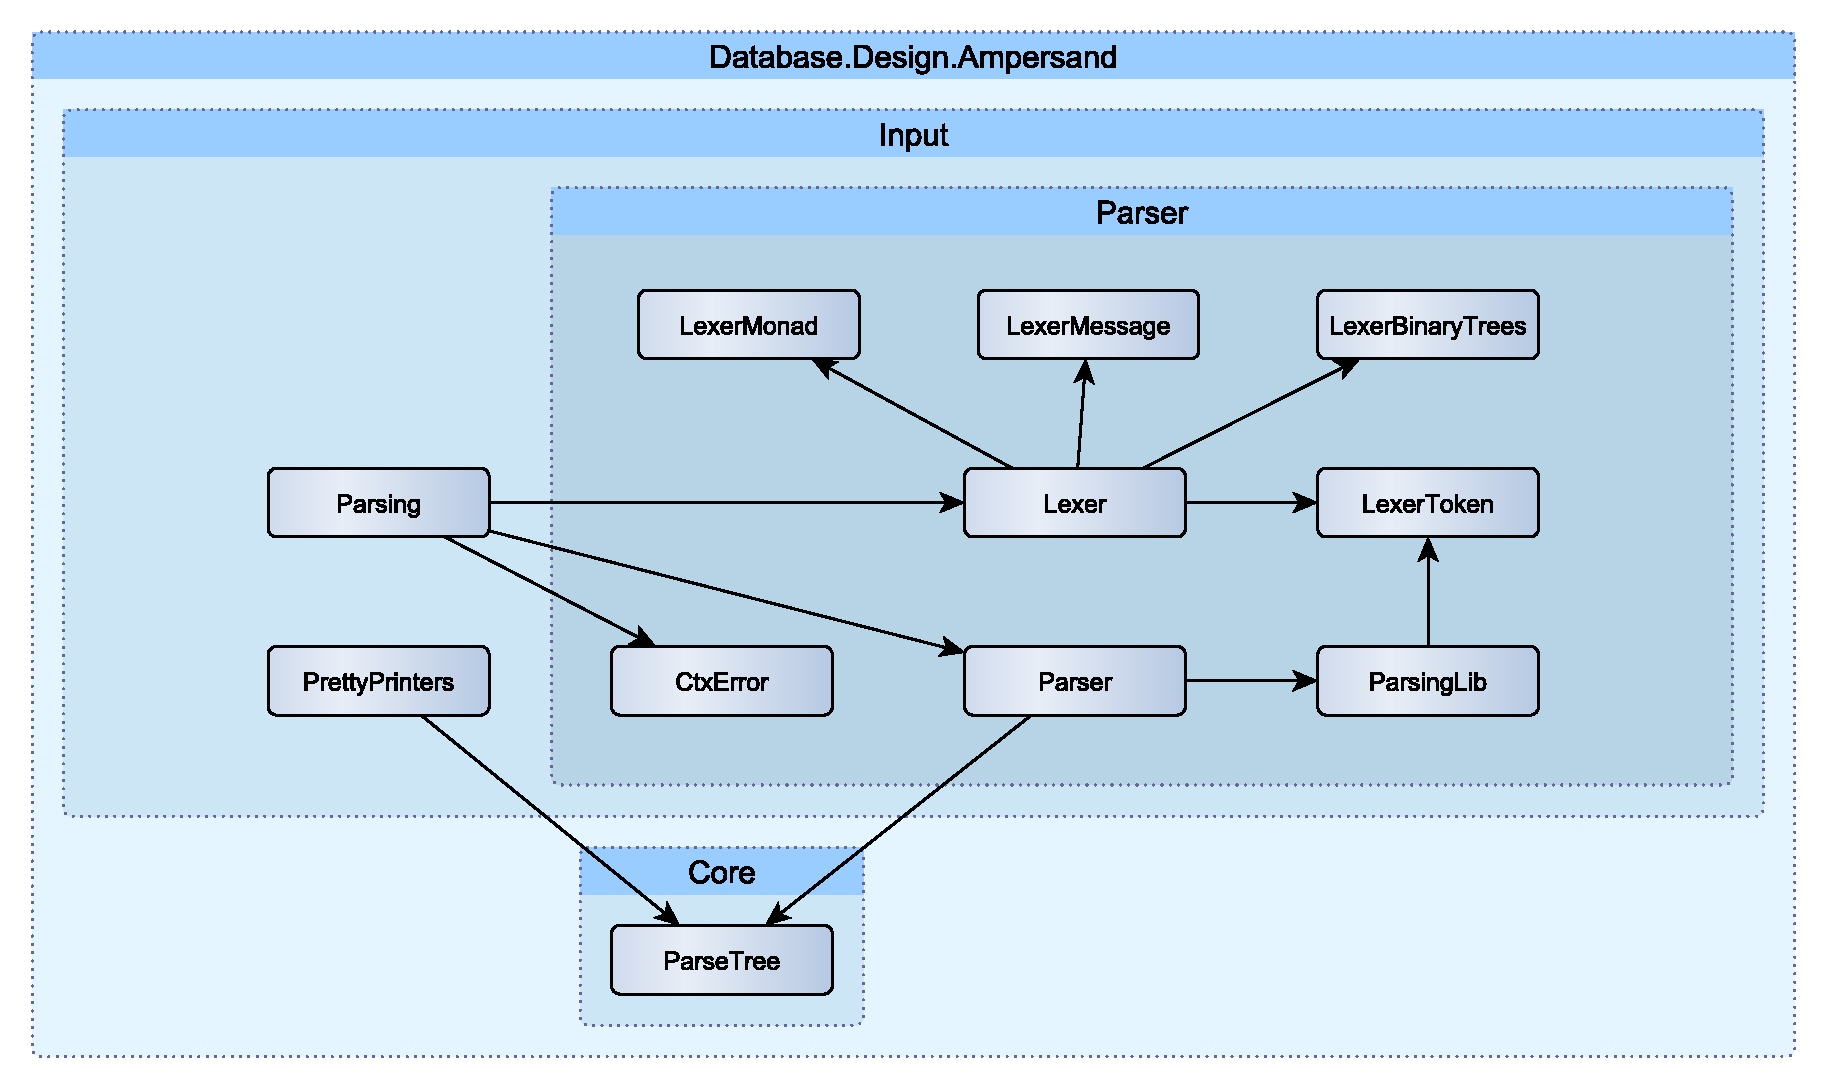
\includegraphics[width=0.7\columnwidth]{Figures/ParserModules}
    \caption{The modules relevant for the parser and their relationships}
    \label{fig:ParserModules}
  \end{figure}%
  Each module has the following responsibilities:
  %
  \begin{description}
    \item[Parsing] module that implements the interface of the parser with the rest of the system.
      It is responsible for reading the input files, calling the lexer and the parser and returning a parse tree as result (or a parse error).

    \item[Parser] module responsible for executing the parsing itself.
      It accepts the tokens that are allowed in each grammar production and generates the corresponding parse tree.
      The parser is described in \autoref{design:new-parser}.
      
    \item[ParsingLib] library that contains several useful functions to assist the parser, e.g. token recognition.
      These functions are not depending on the specific grammar rules.
      
    \item[ParseTree] external module containing the parse tree data structures.
      Only details of this module have been changed during this project (e.g. field ordering).
    
    \item[PrettyPrinters] contains the \texttt{Pretty} class and the functions responsible for printing the parse tree to ADL scripts in a `pretty' way.
    
    \item[CtxError] contains the data structures responsible for the parse errors and their location.
      This module has not been refactored as a part of this project.
    
    \item[Lexer/LexerToken] modules responsible for recognizing the input characters and converting them to tokens.
      The new lexer, together with its sub-modules, is described in \autoref{design:new-lexer}.
  \end{description}

% !TEX root = ../Thesis.tex

\subsection{Errors}
\label{analysis:errors}
%TODO: Bastiaan suggests we should try to use the definition of the error manifesto by Yang et al. (page 32 of his doctor)
In this section, we analyze the error messages given by the previous parser.
The results of this analysis are compared with the new parser in \autoref{tests:errors}.

\subsubsection{Error message qualification}
The user friendliness and correctness of an error message is a subjective topic and therefore we need to start with a definition to objectively judge the quality of an error message.
After analyzing the current Ampersand parser error messages, we identified the following objective aspects of an Ampersand parser error message:
%
\begin{description}
	\item [Position]
	Each error messages reports the correct position (file, line number and column) of where the user committed the error.
	\item [Accuracy]
	The accuracy of an error message is measured based upon the following characteristics:
	\begin{enumerate}
		\item	\textbf{\small How does the provided error description outline the discovered error:}
				Providing the user with a good description of the encountered syntax issue will support a fast error resolution.
				When the issue is vaguely described without pinpointing the exact issue, the error resolution will be time consuming.
		\item	\textbf{\small Pinpointing the correct error}:
				An error can lead to multiple subsequent issues.
				These issues are, however, irrelevant for the user and the Ampersand parser should provide the exact origin of the issues.
		\item	\textbf{\small Quality of the hint:}
			The message can provide a hint for a solution together with the error message to support the user with the error resolution.
	\end {enumerate}
    \item[Conciseness]
	Providing a good error description is one thing, but this one message can be hidden between several other error messages that result from the initial error.
	It is unlikely that users will easily find the exact originating issue in their source file when they are overwhelmed with a multitude of error messages. % using plural to avoid repeating his/her
\end {description}
%
Based on these objective properties to judge the quality of the parsing errors, we defined the following criteria to distinguish between good, bad and average (but acceptable) error messages:
%
%TODO: Bastiaan doesn't think there's a main originating error. See his review in page 15.
\begin{description}
	\item [Bad error message] A message is considered to be bad if one of the criteria below is fulfilled:
		\begin{description}
			\item [Position]
			The position has a deviation of more than one line or ten column positions from where the actual error is made.
			\item [Accuracy]~
				\begin{itemize}
					\item 	The provided error description is useless for the user to determine the actual error.
					\item 	The provided error description is not appointing the main, originating error without any correlation towards this main error.
				\end {itemize}
			\item[Conciseness]
			More than distinct three errors are mentioned by the Ampersand parser.
		\end {description}
	\item [Acceptable error message] A message is considered to be of average, but acceptable, quality if one of the criteria below is fulfilled:
		\begin{description}
			\item [Position]
			The position has a deviation between five and ten column positions from where the actual error is made.
			\item [Accuracy]~
				\begin{itemize}
					\item 	The provided error description is not an exact description of the error, but provides 6useful information to discover the actual issue.
					\item 	The provided error description is not appointing the main originating error, but the link to the actual error can be discovered based on the provided information.
					\item 	The provided hint is incorrect.
				\end {itemize}
			\item[Conciseness]
			two or three errors are mentioned by the Ampersand parser.
		\end {description}
		
	\item [Good error message] Any error message that is not bad nor acceptable is good.
\end {description}

\subsubsection{Gathering process}

To gather the necessary input for the as-is analysis, an exhaustive list of all possible error messages is created.
This as-is analysis will be used as a reference base to verify the implementation of the new error mechanism with Parsec.
The errors are invoked by simulating all possible syntax errors that will invoke an error within the Ampersand parser.
Each syntax statement is therefore manipulated, introducing one specific error per time, and the resulting error message is then recorded together with the actual erroneous statement.
The exact same statements are afterwards pushed through the new parser, making it possible to make a quantitative `before and after' analysis.
Special attention is given to avoid redundant errors that could influence the quantitative analysis. 
An example of such an redundant error is the use of a capital letter in defining a specific reference. 
Although these references are used in several syntax statements, there is only one procedure in the parser to check all references starting with a capital letter.
An improvement in the error message of this check may only be taken into account one time.

\subsubsection{Results}
Based on our error message qualification definition, \autoref{tab:error-messages-analysis} visualizes the results of the as-is analysis.
This analysis clearly confirms the statement that the quality of the error messages is of low quality and that there is a lot of room for improvement.

% Please add the following required packages to your document preamble:
% \usepackage[table,xcdraw]{xcolor}
% If you use beamer only pass "xcolor=table" option, i.e. \documentclass[xcolor=table]{beamer}
\begin{table}[h]
  \centering
	\begin{tabular}{llrlr}
    Error quality  & \multicolumn{2}{c}{Previous parser}     \\
		Good           & 19          & 22,35\%         \\
		Acceptable        & 48          & 56,47\%       \\
		Bad            & 18          & 21,18\%           \\
		\rowcolor[HTML]{BBBBBB}
		\textbf{Total} & \textbf{85} & \textbf{100,00\%} 
	\end{tabular}
  \caption{Error message as-is analysis results}
  \label{tab:error-messages-analysis}
\end{table}

% !TEX root = ../Thesis.tex

\subsection{Grammar}
\label{analysis:grammar}

\subsubsection{Getting the EBNF in good shape}
\dict{EBNF}{Extended Backus-Naur Form}%
\dict{Extended Backus-Naur Form}{Notation technique for documenting context-free grammars}%
The Ampersand grammar is described using the EBNF notation. 
EBNF is a notation technique with the goal to express a context free grammar like Ampersand.
At the beginning of the project, we noticed that the existing EBNF diagram was outdated and not in line anymore with the actual syntax of Ampersand.
As the EBNF is the crucial source of information in building the new parser, the first focus was to update the old EBNF to represent the actual Ampersand Syntax.

Through reverse engineering, we checked all Haskell functions on the actual syntax they implement.
In the source of the new parser, all the grammar expressions are placed above the actual parser function as code annotations to support code maintainability.

\subsubsection{The actual EBNF diagram}
The derived syntax is up to date and visualized using a railroad diagram, an ideal technique to create a visual representation of context free grammars.
Several railroad diagram generators are available on the internet, free of charge.
We used the railroad diagram generator created by Gunter Rademacher, available on \code{\url{http://bottlecaps.de/rr/ui}}.
The generated diagrams with the corresponding EBNF productions are available in the \hyperref[app:docs]{project documentation (appendix)}.

One interesting plus is that during the project we found a bug in the Railroad Diagram Generator.
The tool would crash with the \code{Trm4} expressions.
This bug was reported to the author Gunther Rademacher, who promptly fixed the issue.

% !TEX root = ../Thesis.tex

\subsection{Lexer}
\label{analysis:lexer}
The lexer module is responsible to split up the input stream into tokens.
Tokens are meaningful pieces of the input string that can be recognized by the parser.

The following improvement points were identified after the analysis:
\begin{description}
  \item[Dispersed error messages]
    The error messages produced by the lexer are of good quality.
    Each error message is however defined directly within the corresponding lexer function making the maintenance harder.
  \item[Complex token structure]
    The token structure is complex and confusing (the structure is given below).
    Two values are present in the token, of which one (\code{val1}) is never used.
    There is no distinction between the values used to identify the content of the token and the ones to determine the position of the token, i.e. they are in the same data type.
  \item[Module structuring]
    In the lexer, the actual lexing functions are intermingled with data types, supporting functions and error message texts.
    This makes the lexer harder to understand and to maintain.
  \item[Language support]
    The errors are returned in English only, no multilingual support is available (or easy to implement).
  \item[No support for warnings]
    The lexer can only return errors, warnings are not supported.
  \item[Strings only]
    Token values are stored as strings for all types, with no conversion of values, e.g. integers.
  \item[Lacking documentation]
    There was no documentation available on how the lexer was designed and structured.
\end{description}

\subsubsection{Token structure}
\label{lexer-token}
The old token has the following structure:

\begin{haskell}
data Token = Tok { tp' :: TokenType
                 , val1 :: String
                 , val2 :: String
                 , pos :: !Pos
                 , file :: !Filename
                 }

data TokenType
  = TkSymbol
  | TkVarid
  | TkConid
  | TkKeyword
  | TkOp
  | TkString
  | TkExpl
  | TkAtom
  | TkChar
  | TkInteger8
  | TkInteger10
  | TkInteger16
  | TkTextnm
  | TkTextln
  | TkSpace
  | TkError
  deriving (Eq, Ord)
\end{haskell}
%
%TODO: Add the description as comment in the code, with the explanation that the comments are written by us
The arguments have the following purpose:
\begin{description}
  \item[TokenType]
    Identification of the token type. %, i.e. \code{TkSymbol}, \code{TkVarid}, \code{TkConid}, \code{TkKeyword}, \code{TkOp}, \code{TkString}, \code{TkExpl}, \code{TkAtom}, \code{TkChar}, \code{TkInteger8}, \code{TkInteger10}, \code{TkInteger16}, \code{TkTextnm}, \code{TkTextln}, \code{TkSpace} or \code{TkError}.
  \item[val1]
    This string argument is not used in the lexer.
    In the case of a \code{keyToken} creation, the value is filled in, but we could not find any purpose for this argument.
  \item[val2]
    The actual token content, stored as a string, including the integer values.
  \item[pos]
    Line and column number.
  \item[file]
     Filename in which the token is located.
\end{description}

% !TEX root = ../Documentation.tex

\subsection{Parser (R-M)}
\label{subsec:design-parser}
The mainstream design of the new parser has not changed much.
Basically, each EBNF rule receives its own parser function.
Thanks to the combinator operators, each parsing function also looks very similar to its corresponding EBNF.

The applicative interface is consistently used.
By changing details of the implementation, e.g. the order of the fields in the parse tree, we have made many of the `rebuild' functions unnecessary.
For some parsers the amount of changes necessary in order to remove supporting functions was too large or even impossible with the current parse tree.

Note that in parts of the parser, the function syntax has substituted the record syntax for creating data objects.
This was done only when the code readability could be improved by doing so.

\subsubsection{Parsec}
\label{subsec:design-parsing-lib}
As mentioned earlier, and described in research context document \citenac{parsing}, the new Ampersand parser has been rebuilt with another parsing library, namely Parsec.
However, for the Ampersand developers, the source code of the parser will still look very familiar, thanks to the applicative interface.
For developers, the main differences between Parsec and the uulib are:
\begin{itemize}
  \item Parsec does not backtrack by default.
    In order to enable backtracking, the \texttt{try} function must be used.
    This is described in \autoref{subsec:backtracking}.
  \item Parsec does not try to solve parsing errors.
    The parser stops immediately after the first issue.
    See also the error analysis in \autoref{subsec:design-errors}.
  \item Error messages are customizable by using the \texttt{<?>} operator.
    This is also suggested in \autoref{subsec:design-next-steps}.
  \item Some combinators have a different name, e.g. one must use \texttt{option} instead of \texttt{opt}.
    Assuming the documentation found on Hackage is clear and sufficient, interface differences are not documented here.
\end{itemize}

\subsubsection{Backtracking}
\label{subsec:backtracking}
In order to explain the differences on backtracking behavior between the uulib and Parsec, we quote here Doaitse Swierstra, the author of the uulib \citenac{swierstra-parsec}:
\begin{quote}
\textsl{To understand the subtleties it is important to understand the differences between the try construct in Haskell and the non-greedy parsing strategy used in uu-parsinglib. Effectively the latter is a try which just looks ahead one symbol. In that respect it is less powerful than the try construct from Parsec, in which you specify that a specific construct has to be present completely. And then there is the underlying different overall strategy. Parsec uses a back-tracking strategy with explicit tries to commit, whereas uu-parsinglib uses a breadth-first strategy with an occasional single symbol look-ahead.}
\end{quote}
%
We can therefore conclude that the try-statements in Parsec are undesirable.
However, they are necessary when the grammar is ambiguous.
In this section we explain why each of the remaining try statements are necessary, and how these issues can be resolved:
\begin{description}
  \item[Classify]
    This ambiguity in the grammar arises from the \texttt{Classify} and \texttt{GenDef} productions:
    \begin{quote}
        \texttt{Classify ::= `CLASSIFY' ConceptRef `IS' Cterm}\\
        \texttt{GenDef ::= (`CLASSIFY' | `SPEC') ConceptRef `ISA' ConceptRef}
    \end{quote}
    When the parser encounters \texttt{`CLASSIFY'}, it cannot define whether it found a \texttt{Classify} or a \texttt{GenDef} production.
    Therefore, the parser must consume the keyword and a \texttt{ConceptRef} before consuming either \texttt{`IS'} or \texttt{`ISA'} and determining which production is applicable.
    
    In order to solve this issue, one must choose a different keyword or symbol for each of the productions.
    Another option would be to merge the two statements in the same parser.
    We did not merge the productions because that would make the parser less maintainable.
  
  \item[Role]
    This ambiguity in the grammar arises from the \texttt{RoleRelation} and \texttt{RoleRule} productions:
    \begin{quote}
        \texttt{RoleRelation ::= `ROLE' RoleList `EDITS' NamedRelList}\\
        \texttt{RoleRule ::= `ROLE' RoleList `MAINTAINS' ADLidList}
    \end{quote}
    When the parser encounters \texttt{`ROLE'}, it cannot define whether it is a \texttt{RoleRelation} or a \texttt{RoleRule} production.
    Therefore, the parser must consume the keyword and a \texttt{RoleList} (which may be long) before consuming either \texttt{`MAINTAINS'} or \texttt{`EDITS'} and determining which production is applicable.
    
    In order to solve this issue, one must choose a different keyword for each of the productions, merge the two options to have the same representation in the parse tree, or refactor the parser so that the two options are parsed together.
    We did not merge the productions because that would make the parser less maintainable.
  
  \item[View]
    This ambiguity in the grammar arises from the \texttt{FancyViewDef} and \texttt{ViewDefLegacy} productions:
    \begin{quote}
        \texttt{FancyViewDef ::= `VIEW' Label ConceptOneRefPos `DEFAULT'? `\{' ViewObjList `\}' HtmlView? `ENDVIEW'}\\
        \texttt{ViewDefLegacy ::= (`VIEW' | `KEY') LabelProps ConceptOneRefPos `(' ViewSegmentList `)' }
    \end{quote}
    When the parser encounters \texttt{`VIEW'}, it cannot define whether it found a \texttt{FancyViewDef} or a \texttt{ViewDefLegacy} production.
    In this case, defining which construction is applicable is even more complicated.
    This decision must, in the worst case, be delayed until the parser encounters a \texttt{`\{'} or \texttt{'('}.
    That's because the productions \texttt{Label} and \texttt{LabelProps} are not disjoint, and \texttt{`DEFAULT'} is optional.
    
    In order to solve this issue, we advise to merge or drop the legacy statement.
    
  \item[Multiplicity]
    This ambiguity in the grammar arises from the \texttt{Mult} production:
    \begin{quote}
        \texttt{Mult ::= (`0' | `1') `..' (`1' | `*') | `*' | `1'}
    \end{quote}
    When the parser encounters \texttt{`1'}, it cannot define whether it found the first or the last production.
    The parser must therefore read the next token before choosing the right option.
    
    In order to solve this issue, we advise to refactor the grammar (and the parser) to have the following production:
    \begin{quote}
        \texttt{Mult ::= `0' `..' (`1' | `*') | `1'(`..' (`1' | `*'))? | `*'}
    \end{quote}
    %
    We did not refactor the code in this manner because the \texttt{pMult} parser does more than only parsing: it also changes the representation of the found constructions before creating the parse tree.
  
  \item[Labels and Terms]
    In the productions \texttt{Att} and \texttt{RuleDef}, we see very similar ambiguities:
    \begin{quote}
        \texttt{Att ::= LabelProps? Term}\\
        \texttt{RuleDef ::= `RULE' Label? Rule Meaning* Message* Violation?}
    \end{quote}
    Wherein:
    \begin{quote}
        \texttt{Label ::= ADLid ':'}\\
        \texttt{LabelProps ::= ADLid (`{' ADLidListList `}')? `:'}\\
        \texttt{Rule ::= Term ('=' Term | '|-' Term)?}
    \end{quote}
    And one of the possible productions of \texttt{Term} is:
    \begin{quote}
        \texttt{Term ::= Trm2 ::= Trm3 ::= Trm4 ::= Trm5 ::= Trm6 ::= RelationRef ::= NamedRel ::= Varid Sign?}
    \end{quote}
    While:
    \begin{quote}
        \texttt{ADLid ::= Varid | Conid | String}
    \end{quote}
    
    What happens here is that when the parser encounters a \texttt{Varid}, it cannot define whether it is part of the (optional) \texttt{Label} production or if no \texttt{Label} was given and the \texttt{Varid} is part of a \texttt{Term}/\texttt{NamedRel} production.
    
    Due to the quite complex grammar for the \texttt{Term} production, this issue may severely impact the parser's performance.
    This is probably the most harmful of the ambiguities mentioned.
    However, it can only be solved by adding a symbol before the \texttt{Term} production (e.g. making the `:' non-optional).
\end{description}
%
Please note that in order to have proper backtracking with correct error messages, Parsec may require two try-statements \citenac{try-harmful}.

\begin{landscape}

  \section*{Parse Tree}
  \label{app:parse-tree}
  \addcontentsline{toc}{section}{Parse Tree}
  \begin{figure}[htb!]
    \centering
    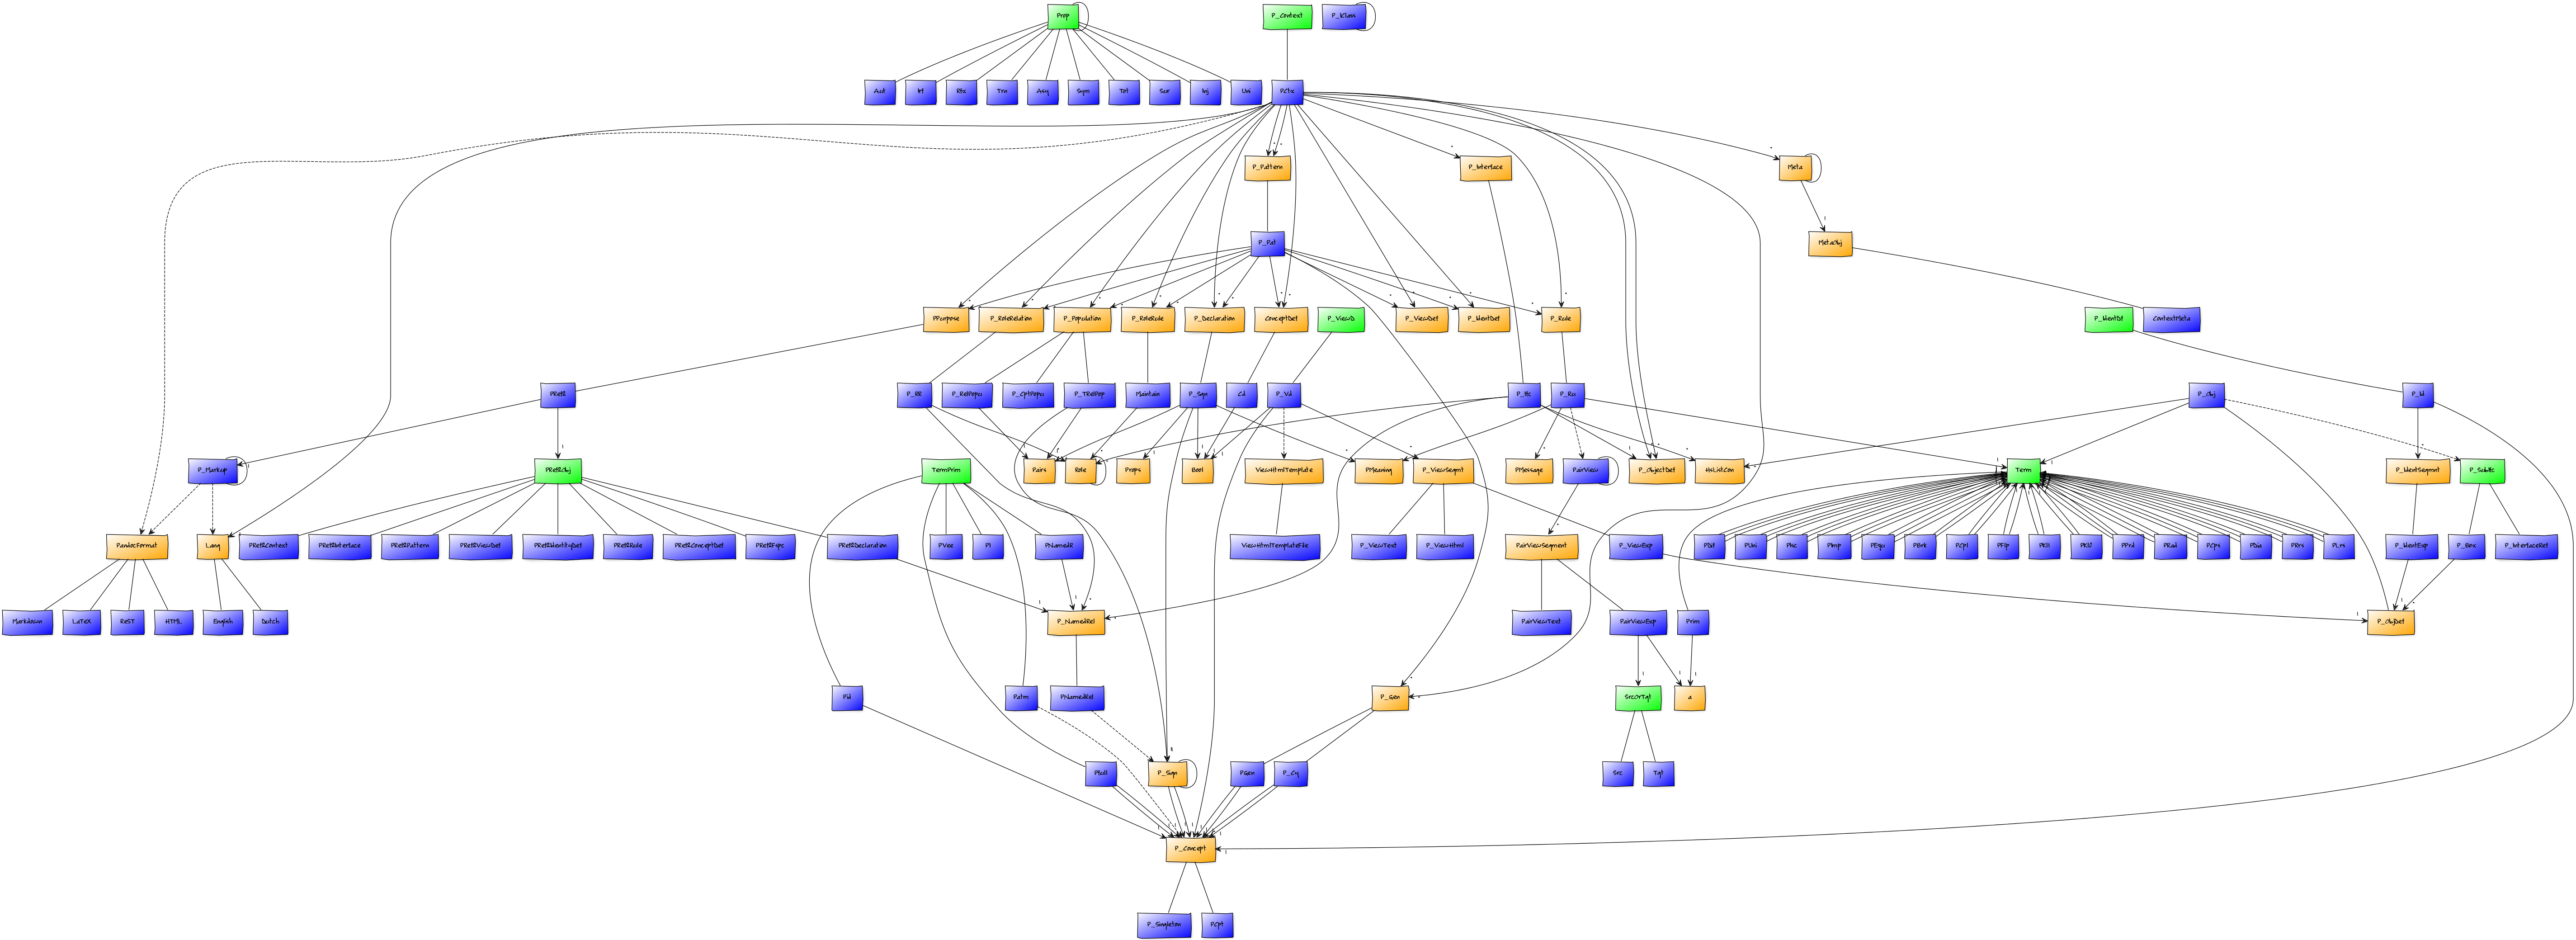
\includegraphics[width=25.4cm]{Figures/GenParseTree}
    \caption[Diagram of the Ampersand parse tree]{
      Diagram of the Ampersand parse tree. \small
      %Data definitions are depicted in green, constructors are depicted in blue and 
      Connections without an arrow represent the data contructors.
      Connections with an arrow also show the multiplicity in the relationship (i.e. 1 or *) or are stripped to represent an optional relationship.
      }
    \label{fig:parse-tree}
  \end{figure}

\end{landscape}

\newpage
% !TEX root = ../Thesis.tex

%beschrijving van het opgeleverde eindproduct, plusminus 15 pagina’s
\section{Design \& Implementation}
\label{sec:design-implementation}
% !TEX root = ../Documentation.tex

\subsection{System overview (R-M)}
  The parser module overview is given in \autoref{fig:ParserModules}.
  \begin{figure}[ht]%
    \centering
    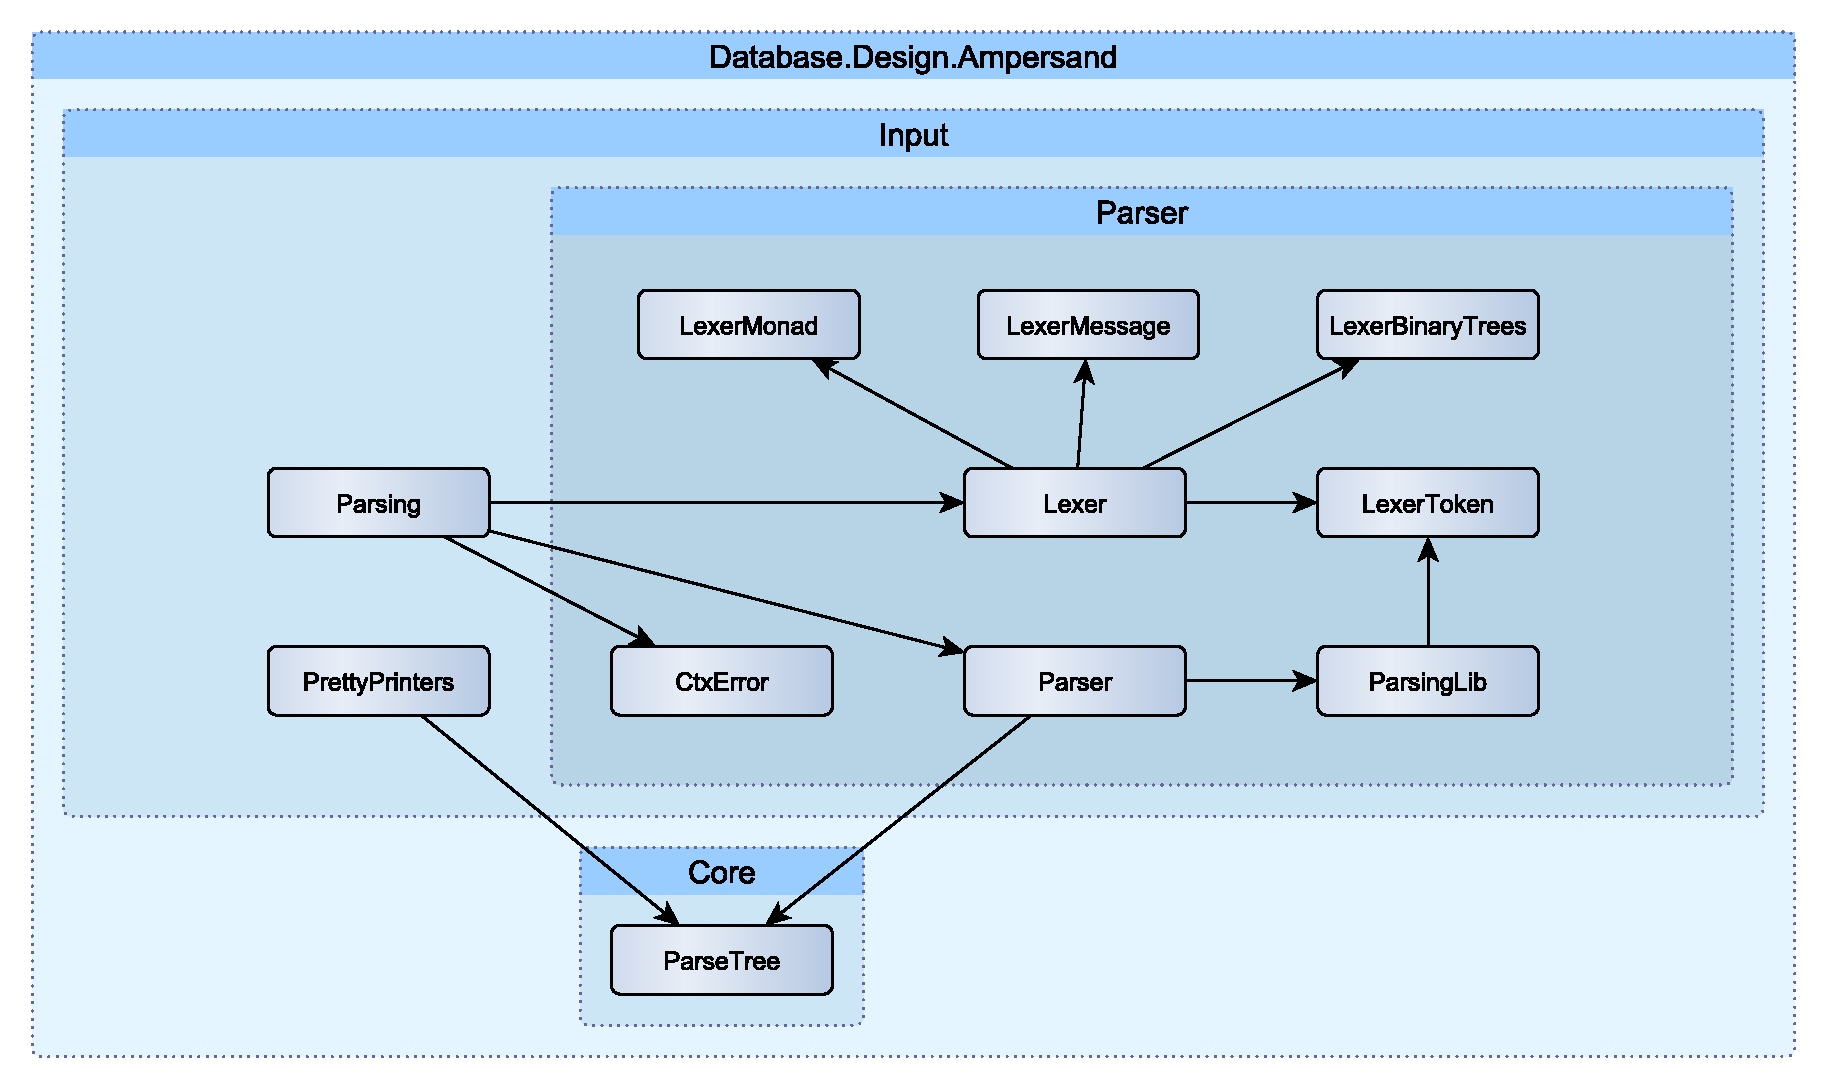
\includegraphics[width=0.7\columnwidth]{Figures/ParserModules}
    \caption{The modules relevant for the parser and their relationships}
    \label{fig:ParserModules}
  \end{figure}%
  Each module has the following responsibilities:
  %
  \begin{description}
    \item[Parsing] module that implements the interface of the parser with the rest of the system.
      It is responsible for reading the input files, calling the lexer and the parser and returning a parse tree as result (or a parse error).

    \item[Parser] module responsible for executing the parsing itself.
      It accepts the tokens that are allowed in each grammar production and generates the corresponding parse tree.
      The parser is described in \autoref{design:new-parser}.
      
    \item[ParsingLib] library that contains several useful functions to assist the parser, e.g. token recognition.
      These functions are not depending on the specific grammar rules.
      
    \item[ParseTree] external module containing the parse tree data structures.
      Only details of this module have been changed during this project (e.g. field ordering).
    
    \item[PrettyPrinters] contains the \texttt{Pretty} class and the functions responsible for printing the parse tree to ADL scripts in a `pretty' way.
    
    \item[CtxError] contains the data structures responsible for the parse errors and their location.
      This module has not been refactored as a part of this project.
    
    \item[Lexer/LexerToken] modules responsible for recognizing the input characters and converting them to tokens.
      The new lexer, together with its sub-modules, is described in \autoref{design:new-lexer}.
  \end{description}

% !TEX root = ../Thesis.tex

\subsection{Software quality factors}
\label{design:software-quality}
In our project plan \citepr{plan} multiple non-functional requirements are included in the project scope.
Improving the code maintainability is one of the most important non-functional requirements.

To assure that these non-functional requirements are correctly addressed, we defined some measures to adhere to during the full project life cycle.

\subsubsection{Documentation}
All important design decisions we made together with the code we delivered need to be documented.
This documentation is needed for the Ampersand team to have a clear insight in the way the new parser is structured and how it is integrated in Ampersand.
The availability of this documentation is crucial for the maintainability of the new parser.
The following documentation is delivered as a result of this ABI project:
%
\begin{description}
  \item[System design]
    A general system overview of the new system, describing the goal and purpose of each module, how it is designed to achieve its goals and how it is integrated in the system architecture.
   The system design is integarted in this thesis document.
  \item[Code annotations]
    Haddock is the de-facto standard for generating Haskell documentation. 
    This documentation generator generates HTML based on the comments in the Haskell source code.
    It is important to remark that Haddock normally only generates documentation of the functions that are exported by each module.
    It is however important that all functions are well documented, including the internal ones, and therefore, the internal functions are documented using regular, non-Haddock, code annotations.
    The code annotations, in the source code, together with the Haddock documentation are delivered as an appendix to this document.
  \item[EBNF comments]
    The EBNF structure is the most important documentation of how the Ampersand syntax is composed and how the parser functions are defined.
    As described in \autoref{analysis:grammar}, the actual EBNF is retrieved through reverse engineering.
    Each parser function corresponds to a specific EBNF syntax rule and this rule is consistently annotated in the code just above the parse function.
  A specific markup (\code{------}) is used to tag the EBNF rules.
  This allows us to automatically extract the EBNF rules from source code and export them to other formats.
\end{description}

\subsubsection{Readability}
  In the as-is analysis of the current parser, we noticed that the code has been through several feature additions over the past years.
  These repetitive small changes reflected in parts of the code which has become too elaborated or sometimes even obsolete.

  Each code statement in the parser and lexer is analyzed by the project team and, where possible, refactored to be as concise as possible.
  The delivered code is now as short as possible without compromising the readability of the code.

  In addition, the code review tool HLint is used.
  This tool provides a full overview of several code optimization suggestions that can further optimize the readability of the source code. 
  These suggestions cover topics such as redundant brackets, parameter reductions and shortcut notations.
  All HLint warnings regarding the input subsystem are fully addressed before the code is delivered to the customer.
  The HLint report for the delivered code is available in the \hyperref[app:docs]{project documentation (appendix)}.

\subsubsection{Performance}
  Performance is a requirement often made in software engineering projects that is difficult to measure before the software is actually used in a production environment.
  For the new Ampersand parser, we proactively identified the topics that could have an impact on the resulting parsing performance.
  In the design of the new parser, a performance aspect that makes an important difference is the parser backtracking (with the \code{try} function).
  Several refactorings in the grammar are carried through to avoid the use of the \code{try} function. 
  A full list of remaining backtracking productions, together with our suggestions how to solve them, is provided in section \autoref{design:backtracking}.

% !TEX root = ../Thesis.tex

\subsection{New Lexer}
\label{design:new-lexer}

\subsubsection{The rationale behind the new lexer}
In the design of the new Ampersand parser, the first decision to tackle is whether to keep the existing scanner/lexer or to implement a new one.
In the analysis of the error improvement areas in \autoref{sec:analysis}, the main improvements are identified within the old parser.
The error feedback quality, produced by the scanner module, is higher and therefore, there is no stringent need to re-implement the scanner.
On the other hand, given the aspect that Parsec is identified as the new parser library, keeping the current scanner would result in the utilization of two different libraries providing more of less the same functionality.

The alternative of keeping the existing scanner would deliver a perfect functional solution, but mixing these two libraries would increase the complexity of the solution, thus decreasing the maintainability.
To avoid this decrease in maintainability, the decision is to implement the parser and scanner based on the same library.

During the implementation of the lexer module, replacing the old scanner, additional attention was given to further improve the quality of the error messages.
The scanner module is renamed to lexer to stress the aspect that the principle of lexemes is used in the new scanner.
Lexemes can be seen as the part of a token containing the actual language content besides the actual position information.

The lexer is built based on the existing Helium lexer modules. 
Helium is a Haskell compiler with the main goal of giving user friendly error messages \citeac{helium}.
The lexer module in Helium contains interesting principles such as position monitoring, warnings and easy maintainable error messages.

% !TEX root = ../Documentation.tex

\subsubsection{Lexer structure}
The lexer is the main module, in which the actual lexing is done, and to do so, it uses the following sub-modules:

 \begin{description}
 
    \item[LexerMonad] contains a monad definition that supports lexing with context.
      It tracks for example the location in the input and the warnings that may be generated.
      This module is based on the Helium lexer, without any modifications to the used functions.
      All unused functions are removed to improve the code maintainability.
      
      The following functions or types are used in the Ampersand lexer:
	  \begin{itemize}
		\item \textbf{LexerMonad} is the main monadic type used in the lexer returning an error or a list of tokens together with a list of warnings
		\item \textbf{addPos} is used to trace the position of the token
		\item \textbf{lexerError} to generate lexer error
		\item \textbf{lexerWarning} to generate lexer warnings
		\item \textbf{runLexerMonad} main function to handle the \code{LexerMonad} results 
	  \end{itemize}
	  
    \item[LexerMessage] contains functions to handle errors and warnings from the lexer.
	  Based on the warning/error type and the needed language, \code{LexerMessage} will fetch the correct description of an error or a warning out of the \code{LexerTexts} module.
	  The show functions for the error and warning are maintained in this module.
	  
    \item[LexerTexts] fetches the correct description of an error or a warning out of the \code{LexerTexts} module.
	  The centralization of the error message texts provides an easy entry point for the maintenance of the actual messages as these messages are no longer dispersed over the module functions.
	  
    \item[LexerBinaryTrees] module responsible for searching binary trees in an efficient way, to support the token recognition.
    This is the previously existing \code{UU\_BinaryTrees} module which is renamed to match the used naming structure of the new lexer modules.

    \item[LexerToken] contains the data structure and corresponding show function that represents the input tokens for the lexer.
	
  \end{description}


\subsubsection{New token structure}
Based on the improvement topics mentioned in \autoref{analysis:lexer}, a new token structure is defined.
Each token contains the lexeme: a part of the input string defining the token type and content, plus the position of the token in the input file.
The token structure is defined as follows:

\begin{haskell}
data Token = Tok { tokLex :: Lexeme    -- ^ The lexeme (defined below)
                 , tokPos :: FilePos   -- ^ The file position
                 }

data Lexeme  = LexSymbol      Char     -- ^ Single character
             | LexOperator    String   -- ^ Operator
             | LexKeyword     String   -- ^ Keyword
             | LexString      String   -- ^ String
             | LexExpl        String   -- ^ Explanation
             | LexAtom        String   -- ^ Atom
             | LexDecimal     Int      -- ^ Decimal integer
             | LexOctal       Int      -- ^ Octal integer
             | LexHex         Int      -- ^ Hexadecimal integer
             | LexConId       String   -- ^ Upper case identifier
             | LexVarId       String   -- ^ Lower case identifier
  deriving (Eq, Ord)
\end{haskell}
%
\code{Lexeme} is the combination of the token type and the actual token content, sliced from the input string.
\code{FilePos} is used to keep track of the original position of the lexeme in the input string.

During the lexer processing, the input file is processed sequentially.
All kinds of different accepted constructions are checked in a specific order.
Each time a match is found, the lexeme is extracted from the input string and a token is created.
In the token creation (function \code{returnToken}), the position and the lexeme are grouped into a token, then the next lexer iteration is started.

% !TEX root = ../Thesis.tex

\subsection{Lexer}
\label{analysis:lexer}
The lexer module is responsible to split up the input stream into tokens.
Tokens are meaningful pieces of the input string that can be recognized by the parser.

The following improvement points were identified after the analysis:
\begin{description}
  \item[Dispersed error messages]
    The error messages produced by the lexer are of good quality.
    Each error message is however defined directly within the corresponding lexer function making the maintenance harder.
  \item[Complex token structure]
    The token structure is complex and confusing (the structure is given below).
    Two values are present in the token, of which one (\code{val1}) is never used.
    There is no distinction between the values used to identify the content of the token and the ones to determine the position of the token, i.e. they are in the same data type.
  \item[Module structuring]
    In the lexer, the actual lexing functions are intermingled with data types, supporting functions and error message texts.
    This makes the lexer harder to understand and to maintain.
  \item[Language support]
    The errors are returned in English only, no multilingual support is available (or easy to implement).
  \item[No support for warnings]
    The lexer can only return errors, warnings are not supported.
  \item[Strings only]
    Token values are stored as strings for all types, with no conversion of values, e.g. integers.
  \item[Lacking documentation]
    There was no documentation available on how the lexer was designed and structured.
\end{description}

\subsubsection{Token structure}
\label{lexer-token}
The old token has the following structure:

\begin{haskell}
data Token = Tok { tp' :: TokenType
                 , val1 :: String
                 , val2 :: String
                 , pos :: !Pos
                 , file :: !Filename
                 }

data TokenType
  = TkSymbol
  | TkVarid
  | TkConid
  | TkKeyword
  | TkOp
  | TkString
  | TkExpl
  | TkAtom
  | TkChar
  | TkInteger8
  | TkInteger10
  | TkInteger16
  | TkTextnm
  | TkTextln
  | TkSpace
  | TkError
  deriving (Eq, Ord)
\end{haskell}
%
%TODO: Add the description as comment in the code, with the explanation that the comments are written by us
The arguments have the following purpose:
\begin{description}
  \item[TokenType]
    Identification of the token type. %, i.e. \code{TkSymbol}, \code{TkVarid}, \code{TkConid}, \code{TkKeyword}, \code{TkOp}, \code{TkString}, \code{TkExpl}, \code{TkAtom}, \code{TkChar}, \code{TkInteger8}, \code{TkInteger10}, \code{TkInteger16}, \code{TkTextnm}, \code{TkTextln}, \code{TkSpace} or \code{TkError}.
  \item[val1]
    This string argument is not used in the lexer.
    In the case of a \code{keyToken} creation, the value is filled in, but we could not find any purpose for this argument.
  \item[val2]
    The actual token content, stored as a string, including the integer values.
  \item[pos]
    Line and column number.
  \item[file]
     Filename in which the token is located.
\end{description}

% !TEX root = ../Thesis.tex

\subsection{New Parser (R-M)}
\label{design:new-parser}
The mainstream design of the new parser has not changed much.
While the new parser may still be recognizable for the Ampersand developers, several improvements have been made.

As decided during the research for domain \& techniques (see \autoref{domain:parsing}), the parser has been rebuilt with the Parsec combinator library.
Basically, each EBNF rule receives its own parser function.
Thanks to the combinator operators, each parsing function also looks very similar to its corresponding EBNF.

The applicative interface is consistently used.
By changing details of the implementation, e.g. the order of the fields in the parse tree, we have made many of the `rebuild' functions unnecessary.
For some parsers the amount of changes necessary in order to remove supporting functions was too large or even impossible with the current parse tree.

Note that in parts of the parser, the function syntax has substituted the record syntax for creating data objects.
This was done only when the code readability could be improved by doing so.

\subsubsection{Parsec}
\label{design:parsing-lib}
As mentioned earlier, and described in research context document \citenac{parsing}, the new Ampersand parser has been rebuilt with another parsing library, namely Parsec.
However, for the Ampersand developers, the source code of the parser will still look very familiar, thanks to the applicative interface.
For developers, the main differences between Parsec and the uulib are:
\begin{itemize}
  \item Parsec does not backtrack by default.
    In order to enable backtracking, the \texttt{try} function must be used.
    This is described in \autoref{design:backtracking}.
  \item Parsec does not try to solve parsing errors.
    The parser stops immediately after the first issue.
   This way, the user is not overwhelmed with irrelevant information.
    See also the error analysis in \autoref{design:errors}.
  \item Error messages are customizable by using the \texttt{<?>} operator.
    This is also suggested in \autoref{design:next-steps}.
  \item Some combinators have a different name, e.g. one must use \texttt{option} instead of \texttt{opt}.
    Assuming the documentation found on Hackage is clear and sufficient, interface differences are not documented here.
\end{itemize}

\subsubsection{Backtracking}
\label{design:backtracking}
In order to explain the differences on backtracking behavior between the uulib and Parsec, we quote here Doaitse Swierstra, the author of the uulib \citenac{swierstra-parsec}:
\begin{quote}
\textsl{To understand the subtleties it is important to understand the differences between the try construct in Haskell and the non-greedy parsing strategy used in uu-parsinglib. Effectively the latter is a try which just looks ahead one symbol. In that respect it is less powerful than the try construct from Parsec, in which you specify that a specific construct has to be present completely. And then there is the underlying different overall strategy. Parsec uses a back-tracking strategy with explicit tries to commit, whereas uu-parsinglib uses a breadth-first strategy with an occasional single symbol look-ahead.}
\end{quote}
%
We can therefore conclude that try-statements in Parsec are undesirable.
However, they are necessary when the grammar is ambiguous.
In this section we explain why each of the remaining try statements are necessary, and how these issues can be resolved:
\begin{description}
  \item[Classify]
    This ambiguity in the grammar arises from the \texttt{Classify} and \texttt{GenDef} productions:
    \begin{ebnf}
     Classify ::= `CLASSIFY' ConceptRef `IS' Cterm
     GenDef ::= (`CLASSIFY' | `SPEC') ConceptRef `ISA' ConceptRef\end{ebnf}
    When the parser encounters \texttt{`CLASSIFY'}, it cannot define whether it found a \texttt{Classify} or a \texttt{GenDef} production.
    Therefore, the parser must consume the keyword and a \texttt{ConceptRef} before consuming either \texttt{`IS'} or \texttt{`ISA'} and determining which production is applicable.
    
    In order to solve this issue, one must choose a different keyword or symbol for each of the productions.
    Another option would be to merge the two statements in the same parser.
    We did not merge the productions because that would make the parser less maintainable.
  
  \item[Role]
    This ambiguity in the grammar arises from the \texttt{RoleRelation} and \texttt{RoleRule} productions:
    \begin{ebnf}
     RoleRelation ::= `ROLE' RoleList `EDITS' NamedRelList
     RoleRule ::= `ROLE' RoleList `MAINTAINS' ADLidList\end{ebnf}
    When the parser encounters \texttt{`ROLE'}, it cannot define whether it is a \texttt{RoleRelation} or a \texttt{RoleRule} production.
    Therefore, the parser must consume the keyword and a \texttt{RoleList} (which may be long) before consuming either \texttt{`MAINTAINS'} or \texttt{`EDITS'} and determining which production is applicable.
    
    In order to solve this issue, one must choose a different keyword for each of the productions, merge the two options to have the same representation in the parse tree, or refactor the parser so that the two options are parsed together.
    We did not merge the productions because that would make the parser less maintainable.
  
  \item[View]
    This ambiguity in the grammar arises from the \texttt{FancyViewDef} and \texttt{ViewDefLegacy} productions:
    \begin{ebnf}
     FancyViewDef ::= `VIEW' Label ConceptOneRefPos `DEFAULT'? `\{' ViewObjList `\}' HtmlView? `ENDVIEW'
     ViewDefLegacy ::= (`VIEW' | `KEY') LabelProps ConceptOneRefPos `(' ViewSegmentList `)'\end{ebnf}
    When the parser encounters \texttt{`VIEW'}, it cannot define whether it found a \texttt{FancyViewDef} or a \texttt{ViewDefLegacy} production.
    In this case, defining which construction is applicable is even more complicated.
    This decision must, in the worst case, be delayed until the parser encounters a \texttt{`\{'} or \texttt{'('}.
    That's because the productions \texttt{Label} and \texttt{LabelProps} are not disjoint, and \texttt{`DEFAULT'} is optional.
    
    In order to solve this issue, we advise to merge or drop the legacy statement.
    
  \item[Multiplicity]
    This ambiguity in the grammar arises from the \texttt{Mult} production:
    \begin{ebnf}
     Mult ::= (`0' | `1') `..' (`1' | `*') | `*' | `1'\end{ebnf}
    When the parser encounters \texttt{`1'}, it cannot define whether it found the first or the last production.
    The parser must therefore read the next token before choosing the right option.
    
    In order to solve this issue, we advise to refactor the grammar (and the parser) to have the following production:
    \begin{ebnf}
     Mult ::= `0' `..' (`1' | `*') | `1'(`..' (`1' | `*'))? | `*'\end{ebnf}
    %
    We did not refactor the code in this manner because the \texttt{pMult} parser does more than only parsing: it also changes the representation of the found constructions before creating the parse tree.
  
  \item[Labels and Terms]
    In the productions \texttt{Att} and \texttt{RuleDef}, we see very similar ambiguities:
    \begin{ebnf}
     Att ::= LabelProps? Term
     RuleDef ::= `RULE' Label? Rule Meaning* Message* Violation?\end{ebnf}
    Wherein:
    \begin{ebnf}
     Label ::= ADLid ':'
     LabelProps ::= ADLid (`{' ADLidListList `}')? `:'
     Rule ::= Term ('=' Term | '|-' Term)?\end{ebnf}
    And one of the possible productions of \texttt{Term} is:
    \begin{ebnf}
     Term ::= Trm2 ::= Trm3 ::= Trm4 ::= Trm5 ::= Trm6 ::= RelationRef ::= NamedRel ::= Varid Sign?\end{ebnf}
    While:
    \begin{ebnf}
     ADLid ::= Varid | Conid | String\end{ebnf}
    
    What happens here is that when the parser encounters a \texttt{Varid}, it cannot define whether it is part of the (optional) \texttt{Label} production or if no \texttt{Label} was given and the \texttt{Varid} is part of a \texttt{Term}/\texttt{NamedRel} production.
    
    Due to the quite complex grammar for the \texttt{Term} production, this issue may severely impact the parser's performance.
    This is probably the most harmful of the ambiguities mentioned.
    However, it can only be solved by adding a symbol before the \texttt{Term} production (e.g. making the `:' non-optional).
\end{description}
%
Please note that in order to have proper backtracking with correct error messages, Parsec may require two try-statements \citenac{try-harmful}.

\subsubsection{Changes to the parse tree}
\label{design:parse-tree}
Improvements in the Ampersand parse tree are out of the scope of this project, because of the potential consequences to the rest of the Ampersand system.
However, during the development of the new parser a few constructions have been changed in order to make the parser more readable and maintainable.
The changes have been mostly in the order of the constructor parameters, and this was done consequently though all Ampersand modules.
The updated parse tree is depicted in the project documentation \citepr{documentation}.

% !TEX root = ../Thesis.tex

\subsection{Errors}
\label{analysis:errors}
%TODO: Bastiaan suggests we should try to use the definition of the error manifesto by Yang et al. (page 32 of his doctor)
In this section, we analyze the error messages given by the previous parser.
The results of this analysis are compared with the new parser in \autoref{tests:errors}.

\subsubsection{Error message qualification}
The user friendliness and correctness of an error message is a subjective topic and therefore we need to start with a definition to objectively judge the quality of an error message.
After analyzing the current Ampersand parser error messages, we identified the following objective aspects of an Ampersand parser error message:
%
\begin{description}
	\item [Position]
	Each error messages reports the correct position (file, line number and column) of where the user committed the error.
	\item [Accuracy]
	The accuracy of an error message is measured based upon the following characteristics:
	\begin{enumerate}
		\item	\textbf{\small How does the provided error description outline the discovered error:}
				Providing the user with a good description of the encountered syntax issue will support a fast error resolution.
				When the issue is vaguely described without pinpointing the exact issue, the error resolution will be time consuming.
		\item	\textbf{\small Pinpointing the correct error}:
				An error can lead to multiple subsequent issues.
				These issues are, however, irrelevant for the user and the Ampersand parser should provide the exact origin of the issues.
		\item	\textbf{\small Quality of the hint:}
			The message can provide a hint for a solution together with the error message to support the user with the error resolution.
	\end {enumerate}
    \item[Conciseness]
	Providing a good error description is one thing, but this one message can be hidden between several other error messages that result from the initial error.
	It is unlikely that users will easily find the exact originating issue in their source file when they are overwhelmed with a multitude of error messages. % using plural to avoid repeating his/her
\end {description}
%
Based on these objective properties to judge the quality of the parsing errors, we defined the following criteria to distinguish between good, bad and average (but acceptable) error messages:
%
%TODO: Bastiaan doesn't think there's a main originating error. See his review in page 15.
\begin{description}
	\item [Bad error message] A message is considered to be bad if one of the criteria below is fulfilled:
		\begin{description}
			\item [Position]
			The position has a deviation of more than one line or ten column positions from where the actual error is made.
			\item [Accuracy]~
				\begin{itemize}
					\item 	The provided error description is useless for the user to determine the actual error.
					\item 	The provided error description is not appointing the main, originating error without any correlation towards this main error.
				\end {itemize}
			\item[Conciseness]
			More than distinct three errors are mentioned by the Ampersand parser.
		\end {description}
	\item [Acceptable error message] A message is considered to be of average, but acceptable, quality if one of the criteria below is fulfilled:
		\begin{description}
			\item [Position]
			The position has a deviation between five and ten column positions from where the actual error is made.
			\item [Accuracy]~
				\begin{itemize}
					\item 	The provided error description is not an exact description of the error, but provides 6useful information to discover the actual issue.
					\item 	The provided error description is not appointing the main originating error, but the link to the actual error can be discovered based on the provided information.
					\item 	The provided hint is incorrect.
				\end {itemize}
			\item[Conciseness]
			two or three errors are mentioned by the Ampersand parser.
		\end {description}
		
	\item [Good error message] Any error message that is not bad nor acceptable is good.
\end {description}

\subsubsection{Gathering process}

To gather the necessary input for the as-is analysis, an exhaustive list of all possible error messages is created.
This as-is analysis will be used as a reference base to verify the implementation of the new error mechanism with Parsec.
The errors are invoked by simulating all possible syntax errors that will invoke an error within the Ampersand parser.
Each syntax statement is therefore manipulated, introducing one specific error per time, and the resulting error message is then recorded together with the actual erroneous statement.
The exact same statements are afterwards pushed through the new parser, making it possible to make a quantitative `before and after' analysis.
Special attention is given to avoid redundant errors that could influence the quantitative analysis. 
An example of such an redundant error is the use of a capital letter in defining a specific reference. 
Although these references are used in several syntax statements, there is only one procedure in the parser to check all references starting with a capital letter.
An improvement in the error message of this check may only be taken into account one time.

\subsubsection{Results}
Based on our error message qualification definition, \autoref{tab:error-messages-analysis} visualizes the results of the as-is analysis.
This analysis clearly confirms the statement that the quality of the error messages is of low quality and that there is a lot of room for improvement.

% Please add the following required packages to your document preamble:
% \usepackage[table,xcdraw]{xcolor}
% If you use beamer only pass "xcolor=table" option, i.e. \documentclass[xcolor=table]{beamer}
\begin{table}[h]
  \centering
	\begin{tabular}{llrlr}
    Error quality  & \multicolumn{2}{c}{Previous parser}     \\
		Good           & 19          & 22,35\%         \\
		Acceptable        & 48          & 56,47\%       \\
		Bad            & 18          & 21,18\%           \\
		\rowcolor[HTML]{BBBBBB}
		\textbf{Total} & \textbf{85} & \textbf{100,00\%} 
	\end{tabular}
  \caption{Error message as-is analysis results}
  \label{tab:error-messages-analysis}
\end{table}

% !TEX root = ../Documentation.tex

\subsection{Next steps (R-M)}
Although we believe the new parser is a large step forward, we also recognize that there are still improvements to be made.

Ampersand is growing and changing in a fast pace.
This is a direct consequence of a project involved with research and active development.
In such projects, it is often impossible to predict which functionalities will be necessary and to design the domain-specific language accordingly beforehand.

As expected we see that most of the remaining issues are related to the grammar ambiguities that force backtracking.
Also the parse tree is not consistently designed.
These issues are mentioned in \autoref{design:next-steps}.
Other improvements are also possible in the test framework delivered.
Those are mentioned in \autoref{tests:next-steps}.


\newpage
% !TEX root = ../Documentation.tex

\section{Test Report}
\label{sec:tests}

\subsection{Test suite}
  Together with the new parser, a test suite has been developed.
  This test suite has been used to verify the performance and correctness of the new parser.
  The source code can be found in the folder \texttt{src/Database/Design/Ampersand/Test} within the Ampersand repository.

  The test suite runs in three steps, which are depicted in \autoref{fig:TestModules}.
  Each of the modules are described in the following subsection.
  %
  \begin{figure}[ht]%
    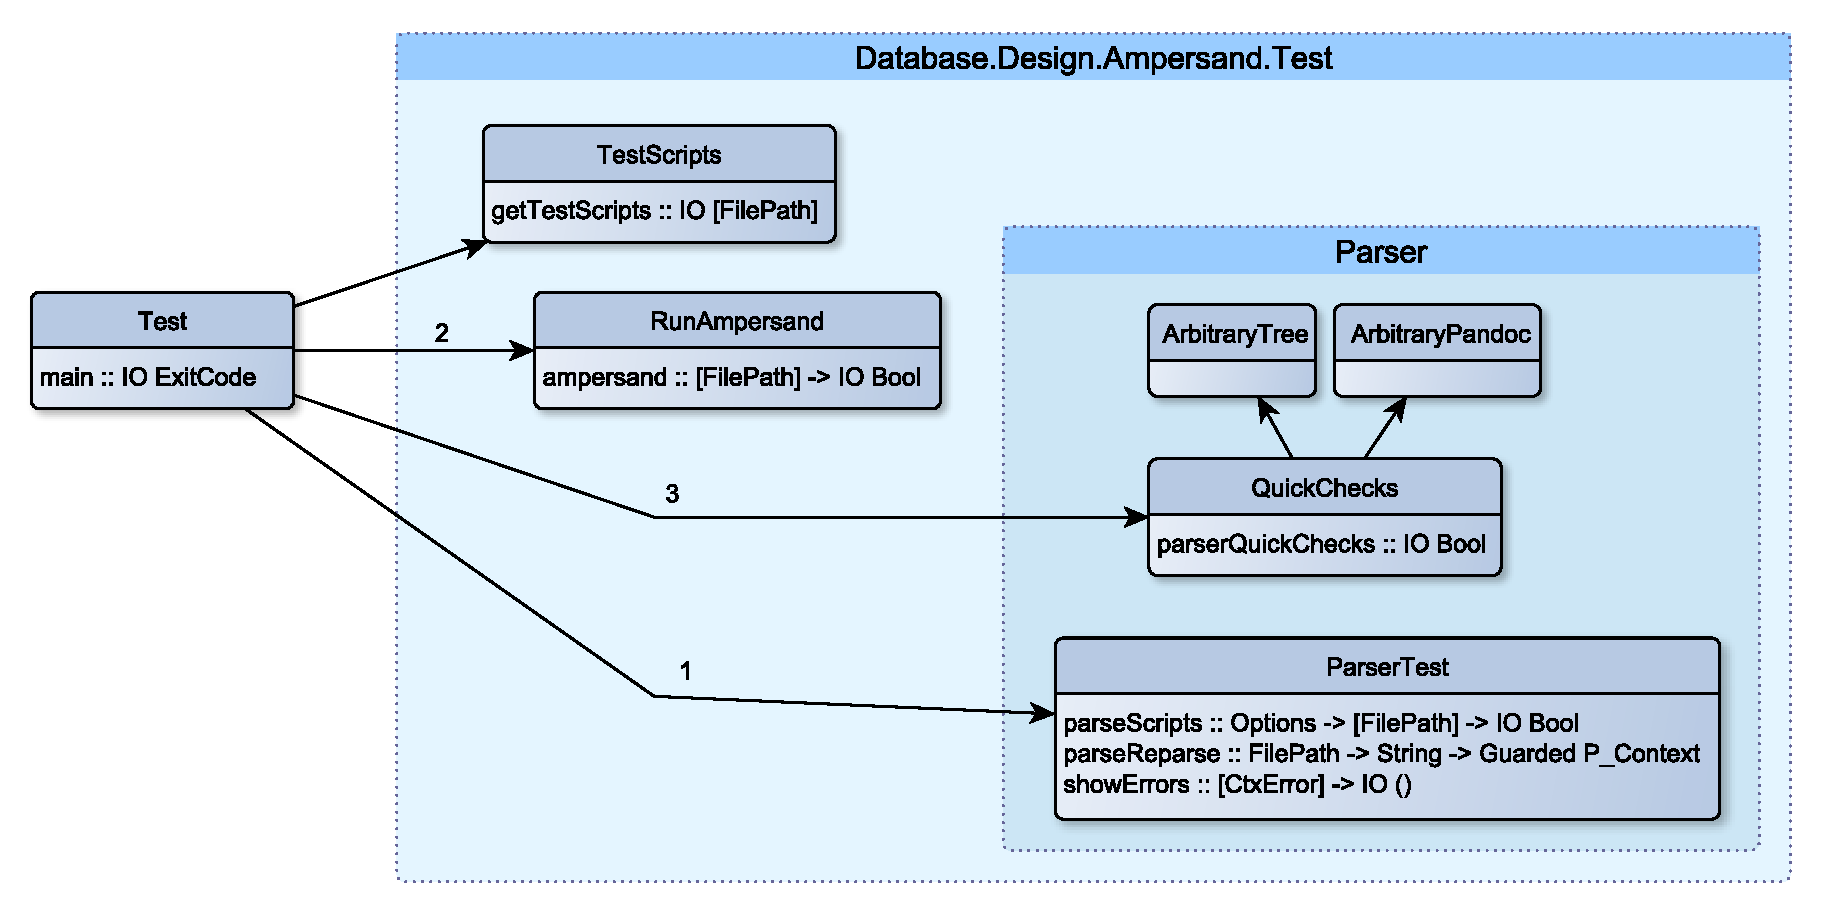
\includegraphics[width=\columnwidth]{Figures/TestModules}
    \caption{Test suite modules with their exported functions}
    \label{fig:TestModules}
  \end{figure}%

  \subsubsection{Modules}
  \label{subsec:test-modules}
  In this section a short description of each module is given:%
  %
  \begin{description}
    \item[Test] contains the \texttt{main} method that can be executed to run the test suite.
      The \texttt{main} function calls each of the other modules in sequence, stopping if any of them returns \texttt{False}.
      When all tests have been successful, the return code is \texttt{ExitSuccess}.
      Otherwise, the return code is naturally \texttt{ExitFailure}.
    
    \item[TestScripts] retrieves a list of scripts that can be used for the different tests.
      It searches for tests within the folder \texttt{ArchitectureAndDesign}, and contains a list of scripts from the \texttt{ampersand-models} repository, that can be changed at a later moment if wished.
      Note that all the ADL-scripts listed in this section must be correct for the parser and the type checker.
    
    \item[ParserTest] exports three functions that are the core of testing the parser:
      \begin{itemize}
        \item \texttt{parseScripts} receives a list of files to parse, and checks that every file can be parsed successfully.
        \item \texttt{parseReparse} tries to parse a file, and if sucessfull, pretty-prints the result and parses it again.
        \item \texttt{showErrors} prints the given parse errors to the output.
      \end{itemize}
    
    \item[RunAmpersand] receives a list of files, and checks that every file can be executed successfully by Ampersand.
      This tests thus not only the parser, but also the interface between the parser and the type checker, as the rest of the Ampersand chain.
    
    \item[QuickChecks] generates random parse tree structures and generates the corresponding ADL-script by pretty printing the parse tree.
      This ADL-script is then fed back to the parser through the \texttt{parseReparse} function, to verify that the parser can accept any random input.
      More information on the quick checks is given in subsection~\ref{subsec:quick-check}.
    
    \item[ArbitraryTree] is a support module that gives \texttt{Arbitrary} instances to all parse-tree structures.
      This is used by QuickCheck as described in subsection~\ref{subsec:quick-check}.
    
    \item[ArbitraryPandoc] contains \texttt{Arbitrary} instances to the Pandoc data types.
      This file has not been developed in this project, but copied from the \texttt{jgm/pandoc} project with the GPL license.
  \end{description}

  \subsubsection{QuickCheck and pretty printing}
  \label{subsec:quick-check}
  The most innovative part of the test suite is the use of random structures to test the parser.
  In this section we describe how this generation is implemented.
  
  The main role in the generation of random structures is played by the support library QuickCheck, which has been added to the Ampersand project.
  QuickCheck is able to generate any data structure randomly.
  However, since the parse tree is a custom structure that must obey specific rules, QuickCheck requires the specification of these rules by instances of the \texttt{Arbitrary} class.
  
  Every data structure in the parse tree has received an \texttt{Arbitrary} instance used for test purposes.
  The instances can be found in the module \texttt{Database.Design.Ampersand.Test.Parser\-.ArbitraryTree}, as described in subsection~\ref{subsec:test-modules}.
  
  After generating the random parse trees, the test suite needs to convert them to ADL-scripts.
  The conversion of parse tree to source code is also known as pretty printing.
  As the pretty printing is seen as part of the parse tree, it is not included in the Test modules, but is part of the input subsystem.
  The pretty printing instances are found in the module \texttt{Database.Design.Ampersand.ADL1.PrettyPrinters}.
  This module makes use of the library \texttt{Text.PrettyPrint.Leijen}, that outlines the output so it is indeed `pretty'.
  
  Now that the ADL source is available, the parser is executed.
  The result of the parser is checked to be equal to the generated tree by the property \texttt{prop\_pretty}.
  The property is currently tested for 64 generated parse trees in the test suite.
  If the test fails for any generated structure, the test suite fails with an appropriate error.
  
  \subsubsection{Running the tests}
  During the parser development, the \texttt{main} function of the parser tests has been executed manually, through a batch file.
  This is mainly done because the project team did not have access to the Sentinel server, and no documentation was available on how to run Sentinel locally in a Windows machine.
  However, now that the parser is being delivered, it should be integrated with the other existing Ampersand/Sentinel tests.
  We leave the option open for the Ampersand development team to either add the Sentinel jobs to this test suite, or to add the parser test suite to the Sentinel jobs.
  
\subsection{Errors}
  Since evaluating the quality of error messages is manual work, the errors have not been included in the test suite.
  TODO: Give Maarten's findings on how the errors have improved. Maybe the tables should be an attachment, but the summary should be here.

\subsection{Next steps}
  In this section we name a couple changes that can be done in the test suite in the future:
  \begin{description}
    \item[Sentinel] During the development of the new parser, we worked in a separate fork.
      Our changes were not being tested in the Ampersand test server (Sentinel).
      Since we did not have access to this server, we developed a separate test suite.
      It may be pertinent to integrate the Sentinel jobs into the test suite or to integrate the test suite into the Sentinel jobs.
    
    \item[Output] Currently, the test suite outputs errors by using the \texttt{Debug.Trace} module.
      From a purely functional perspective, using this module may be undesirable.
      Therefore, the Ampersand team may consider changing the test outputs to use IO with monads in a more functional way.
  \end{description}

\newpage
% !TEX root = ../Thesis.tex

% overzicht van alle topics, samengevat waar mogelijk, die nog als todo staan of waar we verdere verbertering voorstellen
\section{Recommendations}
\label{sec:recommendations}
Although we believe the new parser is a large step forward, we also recognize that there are still improvements to be made.

Ampersand is growing and changing in a fast pace.
This is a direct consequence of a project involved with research and active development.
In such projects, it is often impossible to predict which functionalities will be necessary and to design the domain-specific language accordingly beforehand.

As expected we see that most of the remaining issues are related to the grammar ambiguities that force backtracking.
Also the parse tree is not consistently designed.
These issues are mentioned in \autoref{recommendations:design}.
Other improvements are also possible in the test framework delivered.
Those are mentioned in \autoref{recommendations:tests}.

% !TEX root = ../Documentation.tex

\section{Design}
\label{sec:design}

\subsection{System overview (D)}
  The parser module overview is given in \autoref{fig:ParserModules}.
  Each of the modules are described in the following subsection.
  %
  \begin{figure}[ht]%
    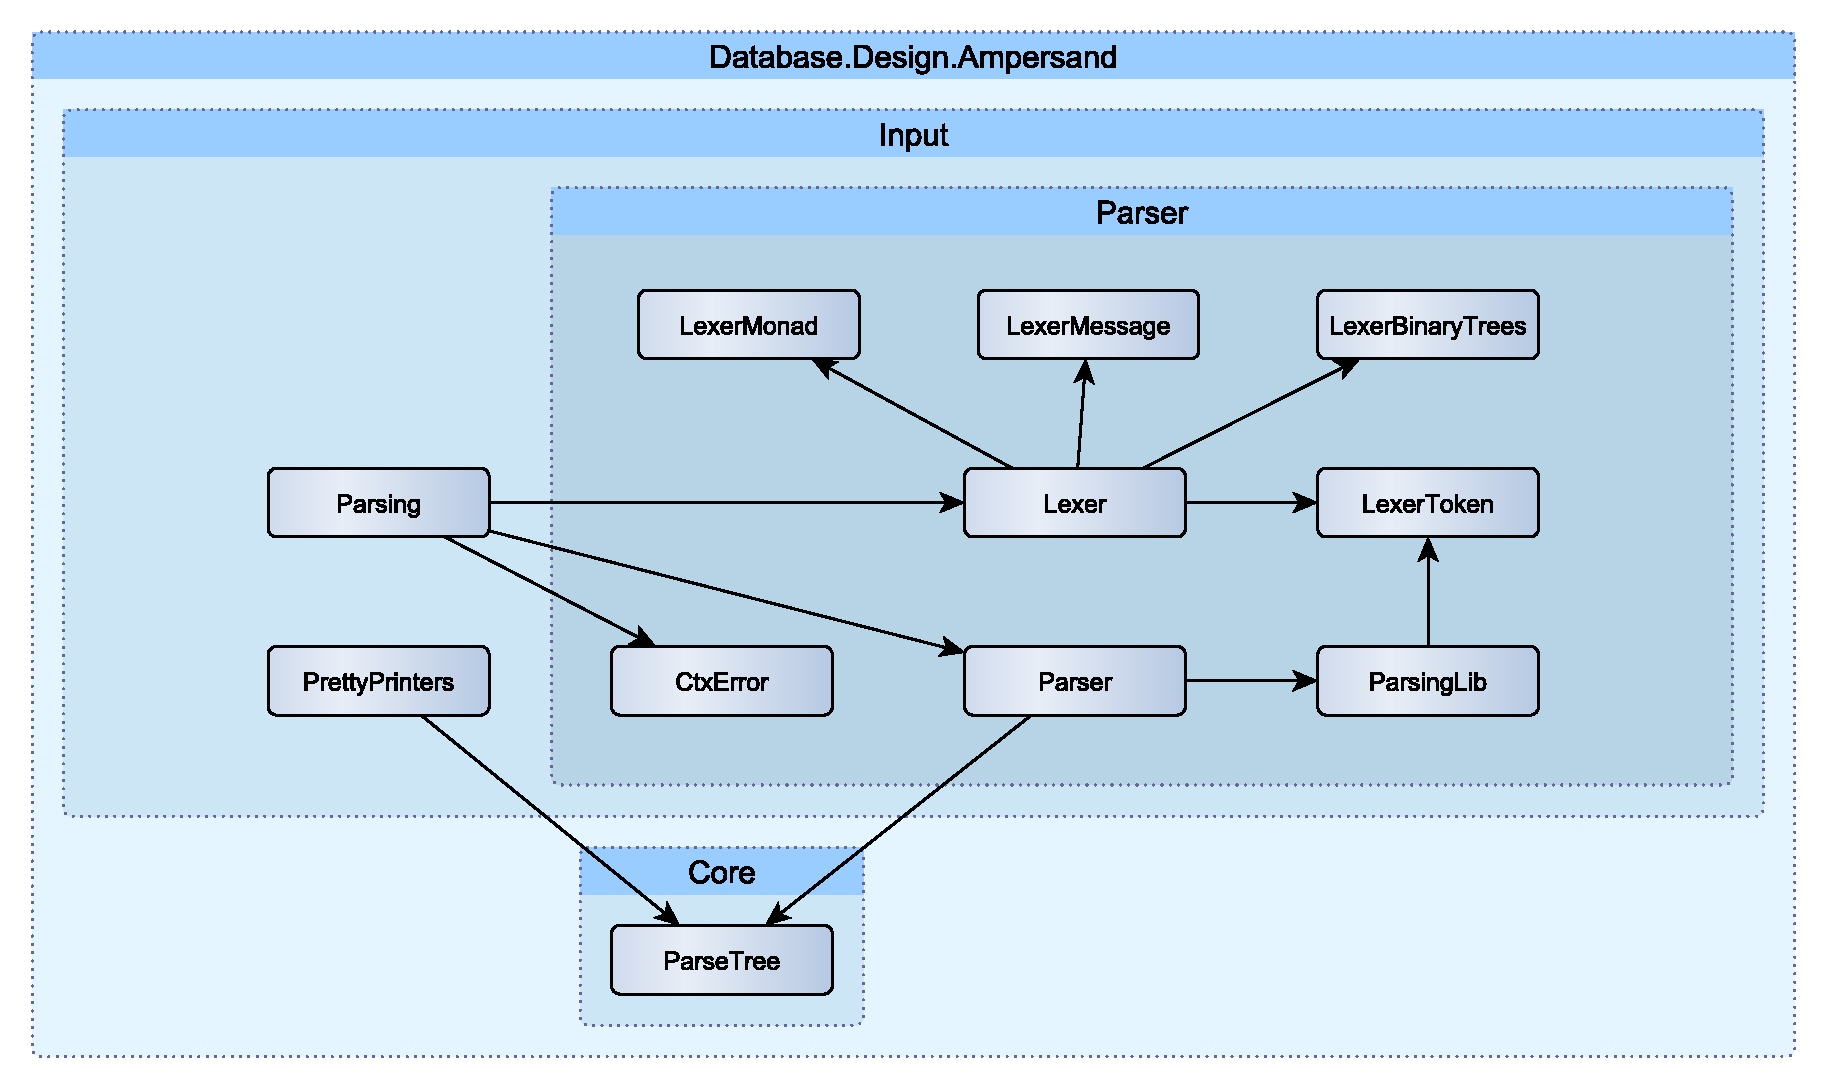
\includegraphics[width=\columnwidth]{Figures/ParserModules}
    \caption{The parser modules and their relationships}
    \label{fig:ParserModules}
  \end{figure}%
  TODO: Add the exported functions to each module.

  \subsubsection{Modules}
  \label{subsec:parser-modules}
  In this section a short description of each module is given:
  %
  \begin{description}
    \item[Parsing] module that implements the interface of the parser with the rest of the system.
      It is responsible for reading the input files, calling the lexer and the parser and returning a parse tree as result (or a parse error).

    \item[Parser] module responsible for executing the parsing itself.
      It accepts the tokens that are allowed in each grammar production and generates the corresponding parse tree.
      The parser is described in \autoref{subsec:design-parser}.
      
    \item[ParsingLib] library that contains several useful functions to assist the parser, e.g. token recognition.
      These functions are not depending on the specific grammar rules.
      
    \item[ParseTree] external module containing the parse tree data structures.
      Only details of this module have been changed during this project (e.g. field ordering).
    
    \item[PrettyPrinters] contains the \texttt{Pretty} class and the functions responsible for printing the parse tree to ADL scripts in a `pretty' way.
    
    \item[CtxError] contains the data structures responsible for the parse errors and their location.
      This module has not been refactored as a part of this project.
    
    \item[Lexer] module responsible for recognizing the input characters and converting them to tokens.
      The lexer, together with its sub-modules, is described in \autoref{subsec:lexer}.
  \end{description}

\subsection{Lexer (M)}
\label{subsec:lexer}
The lexer module is responsible to split up the input stream into tokens.
Tokens are meaningful pieces of the input strings that needs to be kept together together.

\subsubsection{The rationale behind the new lexer}
In the design of the new Ampersand parser, the question arose whether to keep the current scanner or to implement a new one.
After the analysis of the error improvement areas, the main improvements were identified within the actual parser.
The error feedback quality produced by the scanner module was higher and therefore, there was no stringent need to re-implement the scanner.
On the other hand, given the aspect that Parsec was defined as the new Parser library, keeping the current scanner would have resulted in the utilization of 2 different libraries providing more of less the same functionality.
To avoid a decrease in maintainability, the decision is made to implement the parser and scanner based on the same library.
During the implementation of the lexer module, replacing the old scanner, additional attention was given to further improve the quality of the error messages
The scanner module is renamed to the lexer module to stress the aspect that the principle of lexemes is used in the new scanner.

The lexer is build based on the existing Helium lexer modules. 
One of the main goals of this project create a compiler and a dialect of Haskell in which clear error messages were produced. TODO: reference
The Lexer module in Helium contains interesting principles such as position monitoring, warnings and easy maintainable error messages.


\subsubsection{Lexer structure}


The lexer is the main module, in which the actual lexing is done, and to do so, it it using the following sub-modules:

 \begin{description}
 
    \item[LexerMonad] contains a monad definition that supports lexing with context.
      It tracks for example the location in the input and the warnings that may be generated.
	  This module is re-used without any modification out of the  Helium parser.
      The following functions or types are used in the Ampersand lexer:
	  \begin{itemize}
		\item [LexerMonad] is the main monadic type used in the lexer returning an error or a list of tokens together with a list of warnings
		\item [addPos] is used to trace the position of the token
		\item [lexerError] to generate lexer error
		\item [lexerWarning] to generate lexer warnings
		\item [runLexerMonad] main function to handle the LexerMonad results 
	  \end{itemize}
	  
    \item[LexerMessage] contains functions to handle errors and warnings from the lexer.
	  Based on the warning/error type and the needed language, LexerMessage will fetch the correct description of an error or a warning out of the LexerTexts module
	  The show functions for the error and warning are maintained in this module.
	  
    \item[LexerTexts] will fetch the correct description of an error or a warning out of the LexerTexts module.
	  This centralisation provides an easy entry point for the maintenance of the actual messages as the actual messages are no longer dispersed over the module functions.
	  
    \item[LexerBinaryTrees] module responsible for searching binary trees in an efficient way, to support the token recognition.
            This is the existing UU_BinaryTrees module which is renamed to match the used naming structure of the new lexer modules.

    \item[LexerToken] contains the data structure, and corresponding show function, that represents the input tokens for the lexer.
	
  \end{description}

Each token contains a part of the input string together with an identifier, defining the token content, and the position of the token in the input file.
The token structure is defined as follows:

data Token = Tok \{	  tokLex :: Lexeme
                		, tokPos :: FilePos \}

The lexeme is the combination of the token type and the actual token content, sliced from the input string.
FilePos is used to keep track of the original position of the lexeme in the input string.

During the lexer processing, the input file is processed sequentially.
All kind of differentiating formats are checked in a specific order, and each time a match is found, the lexeme is extracted from the input file and the token is created.
In the token creation, function ReturnToken, the position and lexeme is grouped into the actual token and the next nested lexer iteration is launched.


\subsection{Parser (R-M)}
\label{subsec:design-parser}
The mainstream design of the new parser has not changed much.
Basically, each EBNF rule receives its own parser function.
Thanks to the combinator operators, each parsing function also looks very similar to its corresponding EBNF.

The applicative interface is consistently used.
By changing details of the implementation, e.g. the order of the fields in the parse tree, we have made many of the `rebuild' functions unnecessary.
For some parsers the amount of changes necessary in order to remove supporting functions was too large or even impossible with the current parse tree.

Note that in parts of the parser, the function syntax has substituted the record syntax for creating data objects.
This was done only when the code readability could be improved by doing so.

\subsubsection{Parsec}
\label{subsec:design-parsing-lib}
As mentioned earlier, and described in research context document \citenac{parsing}, the new Ampersand parser has been rebuilt with another parsing library, namely Parsec.
However, for the Ampersand developers, the source code of the parser will still look very familiar, thanks to the applicative interface.
For developers, the main differences between Parsec and the uulib are:
\begin{itemize}
  \item Parsec does not backtrack by default.
    In order to enable backtracking, the \texttt{try} function must be used.
    This is described in \autoref{subsec:backtracking}.
  \item Parsec does not try to solve parsing errors.
    The parser stops immediately after the first issue.
    See also the error analysis in \autoref{subsec:design-errors}.
  \item Error messages are customizable by using the \texttt{<?>} operator.
    This is also suggested in \autoref{subsec:design-next-steps}.
  \item Some combinators have a different name, e.g. one must use \texttt{option} instead of \texttt{opt}.
    Assuming the documentation found on Hackage is clear and sufficient, interface differences are not documented here.
\end{itemize}

\subsubsection{Backtracking}
\label{subsec:backtracking}
In order to explain the differences on backtracking behavior between the uulib and Parsec, we quote here Doaitse Swierstra, the author of the uulib \citenac{swierstra-parsec}:
\begin{quote}
\textsl{To understand the subtleties it is important to understand the differences between the try construct in Haskell and the non-greedy parsing strategy used in uu-parsinglib. Effectively the latter is a try which just looks ahead one symbol. In that respect it is less powerful than the try construct from Parsec, in which you specify that a specific construct has to be present completely. And then there is the underlying different overall strategy. Parsec uses a back-tracking strategy with explicit tries to commit, whereas uu-parsinglib uses a breadth-first strategy with an occasional single symbol look-ahead.}
\end{quote}
%
We can therefore conclude that the try-statements in Parsec are undesirable.
However, they are necessary when the grammar is ambiguous.
In this section we explain why each of the remaining try statements are necessary, and how these issues can be resolved:
\begin{description}
  \item[Classify]
    This ambiguity in the grammar arises from the \texttt{Classify} and \texttt{GenDef} productions:
    \begin{quote}
        \texttt{Classify ::= `CLASSIFY' ConceptRef `IS' Cterm}\\
        \texttt{GenDef ::= (`CLASSIFY' | `SPEC') ConceptRef `ISA' ConceptRef}
    \end{quote}
    When the parser encounters \texttt{`CLASSIFY'}, it cannot define whether it found a \texttt{Classify} or a \texttt{GenDef} production.
    Therefore, the parser must consume the keyword and a \texttt{ConceptRef} before consuming either \texttt{`IS'} or \texttt{`ISA'} and determining which production is applicable.
    
    In order to solve this issue, one must choose a different keyword or symbol for each of the productions.
    Another option would be to merge the two statements in the same parser.
    We did not merge the productions because that would make the parser less maintainable.
  
  \item[Role]
    This ambiguity in the grammar arises from the \texttt{RoleRelation} and \texttt{RoleRule} productions:
    \begin{quote}
        \texttt{RoleRelation ::= `ROLE' RoleList `EDITS' NamedRelList}\\
        \texttt{RoleRule ::= `ROLE' RoleList `MAINTAINS' ADLidList}
    \end{quote}
    When the parser encounters \texttt{`ROLE'}, it cannot define whether it is a \texttt{RoleRelation} or a \texttt{RoleRule} production.
    Therefore, the parser must consume the keyword and a \texttt{RoleList} (which may be long) before consuming either \texttt{`MAINTAINS'} or \texttt{`EDITS'} and determining which production is applicable.
    
    In order to solve this issue, one must choose a different keyword for each of the productions, merge the two options to have the same representation in the parse tree, or refactor the parser so that the two options are parsed together.
    We did not merge the productions because that would make the parser less maintainable.
  
  \item[View]
    This ambiguity in the grammar arises from the \texttt{FancyViewDef} and \texttt{ViewDefLegacy} productions:
    \begin{quote}
        \texttt{FancyViewDef ::= `VIEW' Label ConceptOneRefPos `DEFAULT'? `\{' ViewObjList `\}' HtmlView? `ENDVIEW'}\\
        \texttt{ViewDefLegacy ::= (`VIEW' | `KEY') LabelProps ConceptOneRefPos `(' ViewSegmentList `)' }
    \end{quote}
    When the parser encounters \texttt{`VIEW'}, it cannot define whether it found a \texttt{FancyViewDef} or a \texttt{ViewDefLegacy} production.
    In this case, defining which construction is applicable is even more complicated.
    This decision must, in the worst case, be delayed until the parser encounters a \texttt{`\{'} or \texttt{'('}.
    That's because the productions \texttt{Label} and \texttt{LabelProps} are not disjoint, and \texttt{`DEFAULT'} is optional.
    
    In order to solve this issue, we advise to merge or drop the legacy statement.
    
  \item[Multiplicity]
    This ambiguity in the grammar arises from the \texttt{Mult} production:
    \begin{quote}
        \texttt{Mult ::= (`0' | `1') `..' (`1' | `*') | `*' | `1'}
    \end{quote}
    When the parser encounters \texttt{`1'}, it cannot define whether it found the first or the last production.
    The parser must therefore read the next token before choosing the right option.
    
    In order to solve this issue, we advise to refactor the grammar (and the parser) to have the following production:
    \begin{quote}
        \texttt{Mult ::= `0' `..' (`1' | `*') | `1'(`..' (`1' | `*'))? | `*'}
    \end{quote}
    %
    We did not refactor the code in this matter because the \texttt{pMult} parser does more than only parsing: it also changes the representation of the found constructions before creating the parse tree.
  
  \item[Labels and Terms]
    In the productions \texttt{IndAtt}, \texttt{ViewAtt} and \texttt{RuleDef}, we see very similar ambiguities:
    \begin{quote}
        \texttt{IndAtt ::= LabelProps? Term}\\
        \texttt{ViewAtt ::= LabelProps? Term}\\
        \texttt{RuleDef ::= `RULE' Label? Rule Meaning* Message* Violation?}
    \end{quote}
    Wherein:
    \begin{quote}
        \texttt{Label ::= ADLid ':'}\\
        \texttt{LabelProps ::= ADLid (`{' ADLidListList `}')? `:'}\\
        \texttt{Rule ::= Term ('=' Term | '|-' Term)?}
    \end{quote}
    And one of the possible productions of \texttt{Term} is:
    \begin{quote}
        \texttt{Term ::= Trm2 ::= Trm3 ::= Trm4 ::= Trm5 ::= Trm6 ::= RelationRef ::= NamedRel ::= Varid Sign?}
    \end{quote}
    While:
    \begin{quote}
        \texttt{ADLid ::= Varid | Conid | String}
    \end{quote}
    
    What happens here is that when the parser encounters a \texttt{Varid}, it cannot define whether it is part of the (optional) \texttt{Label} production or if no \texttt{Label} was given and the \texttt{Varid} is part of a \texttt{Term}/\texttt{NamedRel} production.
    
    Due to the quite complex grammar for the \texttt{Term} production, this issue may severely impact the parser's performance.
    This is probably the most harmful of the ambiguities mentioned.
    However, it can only be solved by adding a symbol before the \texttt{Term} production (e.g. making the `:' non-optional).
    
    \textbf{TODO: IndAtt and ViewAtt are the same parser.}
\end{description}
%
Please note that in order to have proper backtracking with correct error messages, Parsec may require two try-statements \citenac{try-harmful}.

\subsection{Parse tree (R-M)}
\label{subsec:design-parse-tree}
Improvements in the Ampersand parse tree are out of the scope of this project, because of the potential consequences to the rest of the Ampersand system.
However, during the development of the new parser a few constructions have been changed in order to make the parser more readable and maintainable.
The changes have been mostly in the order of the constructor parameters, and this was done consequently though all Ampersand modules.
The updated parse tree is depicted in the appendices (\autoref{fig:parse-tree}).

\subsection{Errors (M)}
\label{subsec:design-errors}
TODO: show what we've done to improve the errors.

\subsection{Next steps (M)}
\label{subsec:design-next-steps}
TODO: give tips on how to further improve the parser. e.g.:
  - cleanup CtxError, add warnings, use <?> for the errors.
  - reorganize parse tree, e.g. using always Origin as first parameter.
% !TEX root = ../Thesis.tex

% Overzicht van alle mogelijke code verbeteringen die we nog zien
% alle trys worden hierin exhaustief opgenomen
% alle todo's scannen en aanbevelen waar syntaxt optimalisatie hier kan helpen

\subsection{Syntax (M)}
\lipsum[1]

% !TEX root = ../Thesis.tex

% besprekingvan alle mogelijke code verbeteringen die we door ene impact op de parse tree of andere redenen niet behandeld hebben

\subsection{Coding (R-D)}
In the actual parser code, some smaller improvement topics are identified.
Resolving these independent minor topics impacts however the parse tree and therefore, these modifications are still open.
providing a exhaustive overview of these topics in this document would jeopardize the briefness and conciseness of this document.
All improvement topics are however fully documented in the code itself.
% !TEX root = ../Documentation.tex

\section{Test Report}
\label{sec:tests}

\subsection{Test suite}
  Together with the new parser, a test suite has been developed.
  This test suite has been used to verify the performance and correctness of the new parser.
  The source code can be found in the folder \texttt{src/Database/Design/Ampersand/Test} within the Ampersand repository.

  The test suite runs in three steps, which are depicted in \autoref{fig:TestModules}.
  Each of the modules are described in the following subsection.
  %
  \begin{figure}[ht]%
    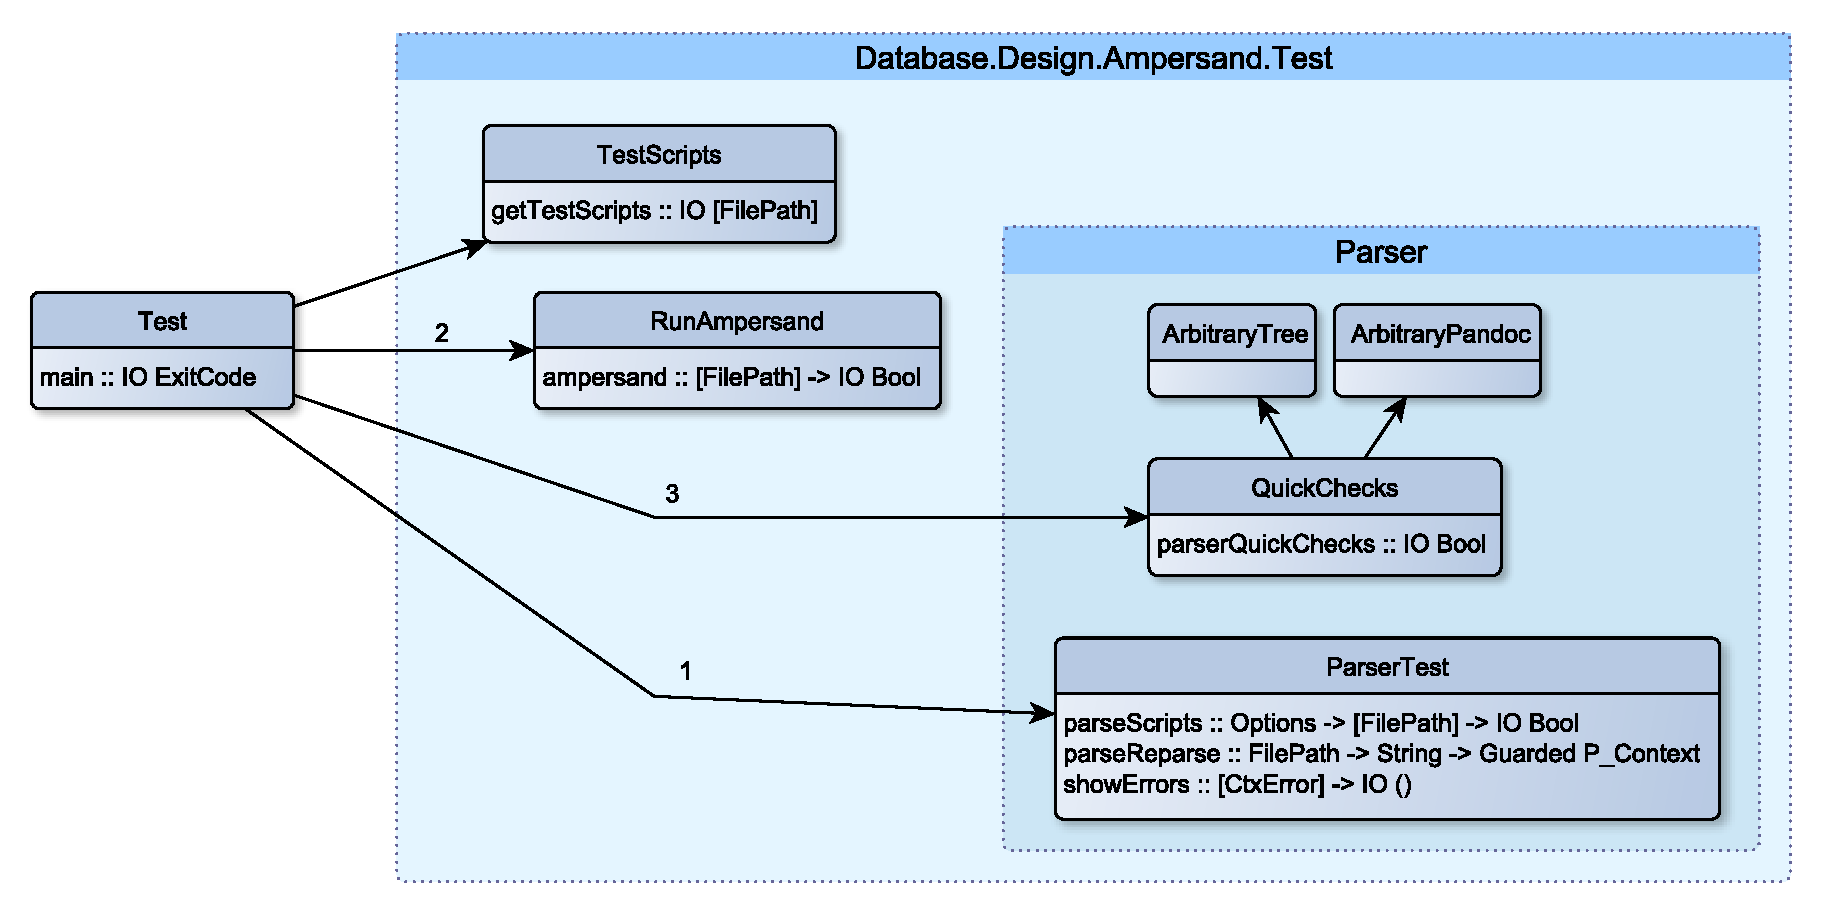
\includegraphics[width=\columnwidth]{Figures/TestModules}
    \caption{Test suite modules with their exported functions}
    \label{fig:TestModules}
  \end{figure}%

  \subsubsection{Modules}
  \label{subsec:test-modules}
  In this section a short description of each module is given:%
  %
  \begin{description}
    \item[Test] contains the \texttt{main} method that can be executed to run the test suite.
      The \texttt{main} function calls each of the other modules in sequence, stopping if any of them returns \texttt{False}.
      When all tests have been successful, the return code is \texttt{ExitSuccess}.
      Otherwise, the return code is naturally \texttt{ExitFailure}.
    
    \item[TestScripts] retrieves a list of scripts that can be used for the different tests.
      It searches for tests within the folder \texttt{ArchitectureAndDesign}, and contains a list of scripts from the \texttt{ampersand-models} repository, that can be changed at a later moment if wished.
      Note that all the ADL-scripts listed in this section must be correct for the parser and the type checker.
    
    \item[ParserTest] exports three functions that are the core of testing the parser:
      \begin{itemize}
        \item \texttt{parseScripts} receives a list of files to parse, and checks that every file can be parsed successfully.
        \item \texttt{parseReparse} tries to parse a file, and if sucessfull, pretty-prints the result and parses it again.
        \item \texttt{showErrors} prints the given parse errors to the output.
      \end{itemize}
    
    \item[RunAmpersand] receives a list of files, and checks that every file can be executed successfully by Ampersand.
      This tests thus not only the parser, but also the interface between the parser and the type checker, as the rest of the Ampersand chain.
    
    \item[QuickChecks] generates random parse tree structures and generates the corresponding ADL-script by pretty printing the parse tree.
      This ADL-script is then fed back to the parser through the \texttt{parseReparse} function, to verify that the parser can accept any random input.
      More information on the quick checks is given in subsection~\ref{subsec:quick-check}.
    
    \item[ArbitraryTree] is a support module that gives \texttt{Arbitrary} instances to all parse-tree structures.
      This is used by QuickCheck as described in subsection~\ref{subsec:quick-check}.
    
    \item[ArbitraryPandoc] contains \texttt{Arbitrary} instances to the Pandoc data types.
      This file has not been developed in this project, but copied from the \texttt{jgm/pandoc} project with the GPL license.
  \end{description}

  \subsubsection{QuickCheck and pretty printing}
  \label{subsec:quick-check}
  The most innovative part of the test suite is the use of random structures to test the parser.
  In this section we describe how this generation is implemented.
  
  The main role in the generation of random structures is played by the support library QuickCheck, which has been added to the Ampersand project.
  QuickCheck is able to generate any data structure randomly.
  However, since the parse tree is a custom structure that must obey specific rules, QuickCheck requires the specification of these rules by instances of the \texttt{Arbitrary} class.
  
  Every data structure in the parse tree has received an \texttt{Arbitrary} instance used for test purposes.
  The instances can be found in the module \texttt{Database.Design.Ampersand.Test.Parser\-.ArbitraryTree}, as described in subsection~\ref{subsec:test-modules}.
  
  After generating the random parse trees, the test suite needs to convert them to ADL-scripts.
  The conversion of parse tree to source code is also known as pretty printing.
  As the pretty printing is seen as part of the parse tree, it is not included in the Test modules, but is part of the input subsystem.
  The pretty printing instances are found in the module \texttt{Database.Design.Ampersand.ADL1.PrettyPrinters}.
  This module makes use of the library \texttt{Text.PrettyPrint.Leijen}, that outlines the output so it is indeed `pretty'.
  
  Now that the ADL source is available, the parser is executed.
  The result of the parser is checked to be equal to the generated tree by the property \texttt{prop\_pretty}.
  The property is currently tested for 64 generated parse trees in the test suite.
  If the test fails for any generated structure, the test suite fails with an appropriate error.
  
  \subsubsection{Running the tests}
  During the parser development, the \texttt{main} function of the parser tests has been executed manually, through a batch file.
  This is mainly done because the project team did not have access to the Sentinel server, and no documentation was available on how to run Sentinel locally in a Windows machine.
  However, now that the parser is being delivered, it should be integrated with the other existing Ampersand/Sentinel tests.
  We leave the option open for the Ampersand development team to either add the Sentinel jobs to this test suite, or to add the parser test suite to the Sentinel jobs.
  
\subsection{Errors}
  Since evaluating the quality of error messages is manual work, the errors have not been included in the test suite.
  TODO: Give Maarten's findings on how the errors have improved. Maybe the tables should be an attachment, but the summary should be here.

\subsection{Next steps}
  In this section we name a couple changes that can be done in the test suite in the future:
  \begin{description}
    \item[Sentinel] During the development of the new parser, we worked in a separate fork.
      Our changes were not being tested in the Ampersand test server (Sentinel).
      Since we did not have access to this server, we developed a separate test suite.
      It may be pertinent to integrate the Sentinel jobs into the test suite or to integrate the test suite into the Sentinel jobs.
    
    \item[Output] Currently, the test suite outputs errors by using the \texttt{Debug.Trace} module.
      From a purely functional perspective, using this module may be undesirable.
      Therefore, the Ampersand team may consider changing the test outputs to use IO with monads in a more functional way.
  \end{description}

% !TEX root = ../Documentation.tex

\subsection{Website and Wiki (M)}
\label{recommendations:website}
\lipsum[8]
%TODO: Write about the state of the wiki and absence of a project website.

\newpage
% !TEX root = ../Parsing.tex

\section{Conclusion}
\label{sec:conclusion}
In \autoref{sec:libraries}, the advice was given to use a combinator library for the new parser of Ampersand.
The main reason to avoid the parser generators is that it is hard to generate useful feedback.
Then, in \autoref{sec:errors}, it was made even more clear that besides generating good messages, those messages should also be customizable.

Therefore, the advice of this research is to use the combinator library that offers the highest level of customization in error messages, Parsec.
Although the uu-parsinglib seems to also be a very good choice, the experiences from the Helium compiler \citeac{helium-parser} should be also considered.
Besides, the Parsec library offers better support.

A list of important consideration points has also been collected through the literature and can be found in \autoref{sec:errors}, more specifically \ref{subsec:errors-ampersand}.
\newpage

% !TEX root = ../Thesis.tex

\appendix
\addcontentsline{toc}{part}{Appendices}
% !TEX root = ../Parsing.tex

\small
\printglossary[style=mcolindex,title=Glossary]
\label{sec:glossary}

\clearpage
% !TEX root = ../Parsing.tex
\addcontentsline{toc}{section}{References}
\label{sec:bibliography}

\begin{thebibliography}{99}

\bibitem{plan}
	Planning for the project `Useful feedback in the Ampersand parser'\\
	Maarten Baertsoen and Daniel S. C. Schiavini\\
	Version 2.0 -- November 29, 2014\\
	\url{http://git.io/NeHuLg}

\bibitem{heeren-error}
	Top Quality Type Error Messages\\
	Bastiaan Heeren\\
	ISBN 90-393-4005-6, September 20, 2005\\
	\url{http://www.open.ou.nl/bhr/phdthesis}

\bibitem{monadic-parsing}
	Functional pearls -- Monadic Parsing in Haskell\\
	Graham Hutton (University of Nottingham) and Erik Meijer (University of Utrecht)\\
	\url{http://www.cs.nott.ac.uk/~gmh/monparsing.pdf}

\bibitem{convert-ebnf}
	 From EBNF to BNF \\
	 Christoph Zenger\\
	 June 4, 2000\\
	 \url{http://lampwww.epfl.ch/teaching/archive/compilation-ssc/2000/part4/parsing/node3.html}

\bibitem{bnf-ebnf}
	BNF and EBNF: What are they and how do they work?\\
	Lars Marius Garshol\\
	August 22, 2008\\
	\url{http://www.garshol.priv.no/download/text/bnf.html}

\bibitem{parser-examples}
	Haskell Parser Examples\\
	Geoff Hulette\\
	August 22, 2014\\
	\url{https://github.com/ghulette/haskell-parser-examples}

\bibitem{hugs-parser}
	Source code of the Hugs parser\\
	March 25, 2007\\
	\url{https://github.com/fuzxxl/Hugs/blob/master/src/parser.y}

\bibitem{ghc-parser}
	GHC: The Parser\\
	December 1, 2014\\
	\url{https://ghc.haskell.org/trac/ghc/wiki/Commentary/Compiler/Parser}
	%\url{https://ghc.haskell.org/trac/ghc/browser/ghc/compiler/parser/Parser.y}
	%https://www.haskell.org/pipermail/haskell-cafe/2013-August/109557.html

\bibitem{helium-parser}
	Helium, for Learning Haskell\\
	Bastiaan Heeren, Daan Leijen, Arjan van IJzendoorn\\
	Utrecht University\\
	\url{http://www.open.ou.nl/bhr/heeren-helium.pdf}
	
\bibitem{gcc-c-parser}
	GCC 4.1 Release Series Changes, New Features, and Fixes\\
	\url{https://gcc.gnu.org/gcc-3.4/changes.html}

\bibitem{gcc-cpp-parser}
	GCC 3.4 Release Series Changes, New Features, and Fixes\\
	\url{https://gcc.gnu.org/gcc-4.1/changes.html}
	
\end{thebibliography}

\end{document}